\documentclass[12pt,a4paper,twoside]{book}
\usepackage{amsmath}
\usepackage{setspace}
\usepackage{geometry}
\usepackage{times}
\usepackage{fancyhdr}
\usepackage[utf8x]{inputenc}
\usepackage{graphicx}
\usepackage{xcolor}
\usepackage{listings}
\graphicspath{ {immagini/} }
\fancyhf{} % clear all header and footers
\renewcommand{\headrulewidth}{0pt} % remove the header rule
\fancyfoot[LE,RO]{\thepage} % Left side on Even pages; Right side on Odd pages
\pagestyle{fancy}
\fancypagestyle{plain}{%
  \fancyhf{}%
  \renewcommand{\headrulewidth}{0pt}%
  \fancyhf[lef,rof]{\thepage}%
}

\usepackage{pdfpages}
\usepackage[italian,english]{babel}
\usepackage[hyphens,spaces,obeyspaces]{url}
\usepackage[hidelinks]{hyperref}
\usepackage[T1]{fontenc}

\usepackage{float}

\usepackage{titlesec}
\titleformat{\chapter}[hang] 
{\normalfont\huge\bfseries}{\chaptertitlename\ \thechapter:}{1em}{} 
\renewcommand{\chaptername}{Capitolo}

\colorlet{punct}{red!60!black}
\definecolor{background}{HTML}{EEEEEE}
\definecolor{delim}{RGB}{20,105,176}
\colorlet{numb}{magenta!60!black}
\lstdefinelanguage{json}{
	basicstyle=\normalfont\ttfamily,
	numbers=left,
	numberstyle=\scriptsize,
	stepnumber=1,
	numbersep=8pt,
	showstringspaces=false,
	breaklines=true,
	frame=lines,
	backgroundcolor=\color{background},
	literate=
	*{0}{{{\color{numb}0}}}{1}
	{1}{{{\color{numb}1}}}{1}
	{2}{{{\color{numb}2}}}{1}
	{3}{{{\color{numb}3}}}{1}
	{4}{{{\color{numb}4}}}{1}
	{5}{{{\color{numb}5}}}{1}
	{6}{{{\color{numb}6}}}{1}
	{7}{{{\color{numb}7}}}{1}
	{8}{{{\color{numb}8}}}{1}
	{9}{{{\color{numb}9}}}{1}
	{:}{{{\color{punct}{:}}}}{1}
	{,}{{{\color{punct}{,}}}}{1}
	{\{}{{{\color{delim}{\{}}}}{1}
	{\}}{{{\color{delim}{\}}}}}{1}
	{[}{{{\color{delim}{[}}}}{1}
	{]}{{{\color{delim}{]}}}}{1},
}



\geometry{a4paper,top=3cm,bottom=3cm,left=3cm,right=3cm,heightrounded,bindingoffset=5mm}
\onehalfspacing
\title{Policy merging in ODRL}
\date{Work in progress}
\author{Gianluca Oldani}

\begin{document}
\maketitle
\tableofcontents
\chapter{ODRL}\label{ODRLChapter}
\section{Il linguaggio}
\subsection{Definizione ed obiettivi}
``L' Open Digital Rights Language (ODRL) è un linguaggio per l'espressione di policy che definisce: un modello dell'informazione flessibile ed interoperativo, un vocabolario e un meccanismo di codifica per la rappresentazione delle istruzioni sull'uso di contenuti o servizi''\cite{ODRLinfMod}.\\
Il linguaggio si pone all'interno dello scenario applicativo nel quale vi è la necessità di definire:
\begin{itemize}
	\item quali azioni siano permesse o proibite su una risorsa. Queste regole possono essere imposte da leggi o direttamente dal possessore dell'asset o servizio;
	\item indicare quali attori interagiscono con le policy definite; in particolare chi può definire le policy e a chi si applicano;
	\item indicare eventuali limiti riguardanti i permessi ed i divieti espressi;.
\end{itemize}
Avere un modello standard per definire questi bisogni dà 2 fondamentali vantaggi:
\begin{itemize}
	\item chi possiede l'asset è in grado di definire in modo chiaro quali siano le azioni che un consumatore può fare, evitanto quindi usi indesiderati;
	\item chi usufruisce dell'asset conosce in modo preciso quali azioni può compiere, evitando così di infrangere regole o leggi.
\end{itemize}
ODRL definisce un modello semantico di permessi, divieti ed obblighi, che può essere usato per descrivere le modalità d'uso di un contenuto. In particolare si cerca di definire i concetti chiave per la creazione di policy machine-readable collegate direttamente all'asset al quale sono associate, permettendo all'utente finale di reperire facilmente informazioni sulla risorsa che utilizza. Quest'ultimo requisito è soddisfatto, poiché ODRL è costruito seguendo i \textit{Linked Data principles}\cite{LinkedDataInfo}:
\begin{itemize}\label{linkedDataPrinc}
\item Utilizzo di URIs come nomi per le risorse;
\item Gli URI sono indirizzi HTTP in modo che si possano cercare informazioni sulle risorse;
\item L'URI deve fornire informazioni utili sulla risorsa;
\item Tra le informazioni, fornire altri URI, in modo che l'utente possa raggiungere altre informazioni.
\end{itemize}
Nonostante questi principi siano più indicati per un'implementazione graph-based, è possibile anche definire utilizzi che non tengano conto dei link tra le varie informazioni.
\subsection{Il modello}\label{modello}
\begin{figure}[H]
	\centering
	\def\svgwidth{\columnwidth}
	\scalebox{0.5}{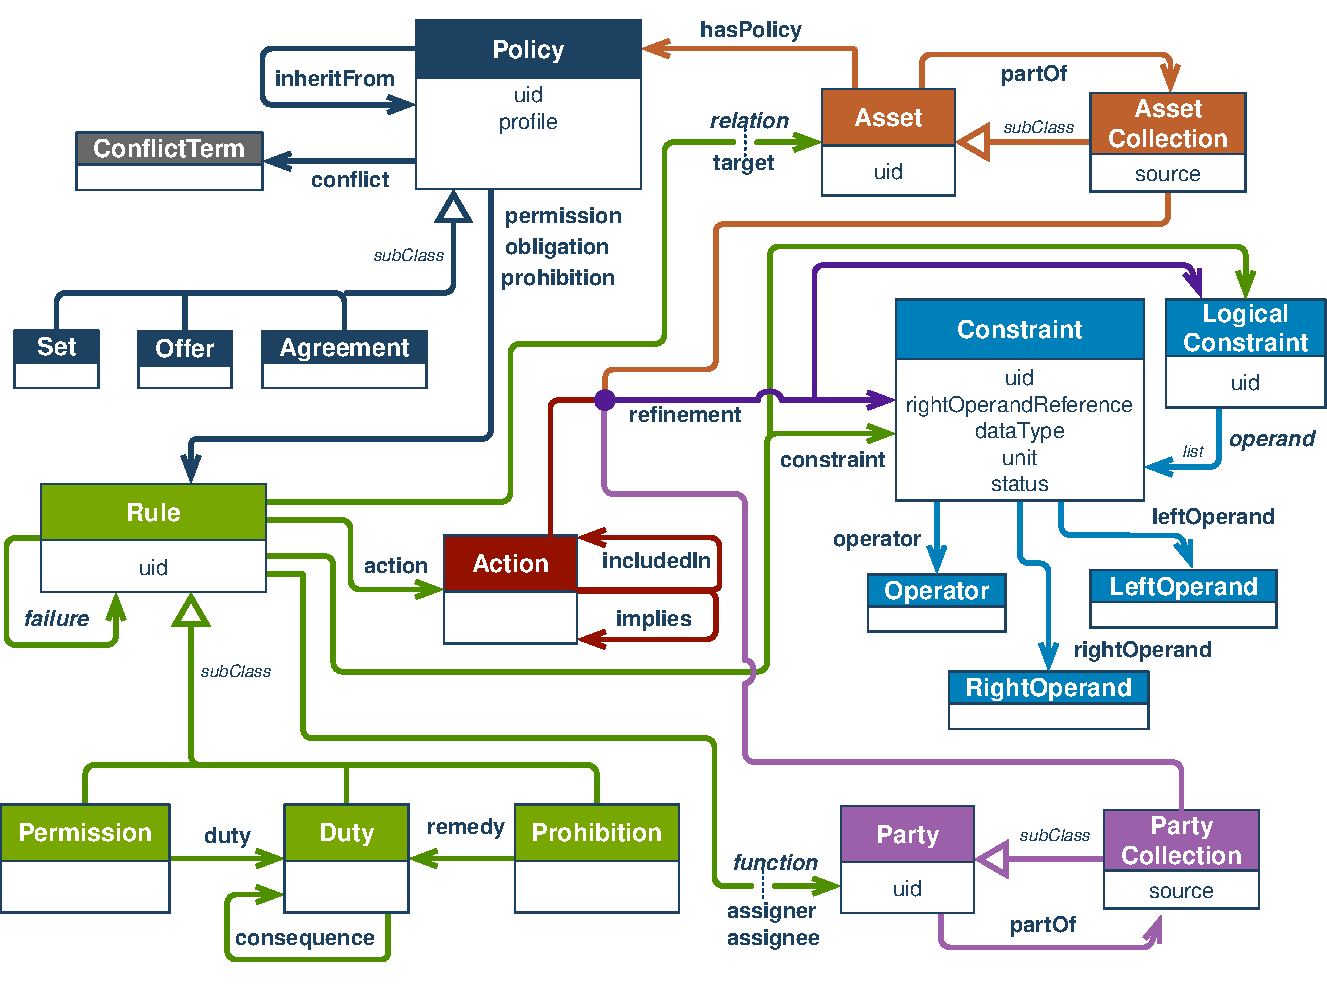
\includegraphics{ODRLModel}}
	
	\caption{Schema del modello ODRL\cite{ODRLinfMod}\label{ODRLModelSchema}}
\end{figure}
Come visibile all'interno dello schema in figura \ref{ODRLModelSchema}, il modello è basato sulle seguenti entità principali:
\begin{itemize}
	\item \textbf{Policy}: un gruppo di una o più regole;
	\item \textbf{Regola}: concetto astratto che racchiude le caratteristiche comuni di \textbf{permesso}, \textbf{divieto}, \textbf{doveri};
	\item \textbf{Asset}: risorsa o collezione di risorse soggette a regole;
	\item \textbf{Azione}: operazione su un asset;
	\item \textbf{Party}: entità o insieme di entità con un certo ruolo in una regola;
	\item \textbf{Limiti}: espressione logica o booleana imposta su azioni, party, asset o regole.
\end{itemize}
\paragraph{Vocabolari}\mbox{}\\
\label{profili}
``L' \textit{ODRL Vocabulary and Expression} descrive i termini usati dalle policy ODRL e come codificarle''\cite{ODRVocab}. All'interno di ODRL, i vocabolari utilizzati per definire i termini all'interno delle policy vengono detti \textbf{profili}, i quali possono essere usati per definire termini che supportano specifiche applicazioni; all'interno di un profilo è possibile, ad esempio, fornire le specifiche riguardanti nuove sottoclassi di termini già presenti nei vocabolari standard di ODRL. I 2 vocabolari principali definiti sono:
\begin{itemize}
	\item \textbf{ODRL Core Vocabulary}: rappresenta la minima espressione di policy supportata;
	\item \textbf{ODRL Common Vocabulary}: arricchisce il vocabolario precedente con un gruppo di azioni generiche, nuove sottoclassi per le policy, ruoli per i party e relazioni tra gli asset.
\end{itemize}
Una delle principali differenze tra i due vocabolari, la si ha all'interno delle \textbf{azioni} che possono essere indicate: nel primo caso si hanno a disposizione solamente 2 azioni \textbf{use} e \textbf{transfer}, nel secondo caso queste 2 azioni vengono estese da diverse azioni figlie, come mostrato in figura \ref{imgUseTransfer}

\begin{figure}[H]
	\centering
	\def\svgwidth{\columnwidth}
	\scalebox{0.35}{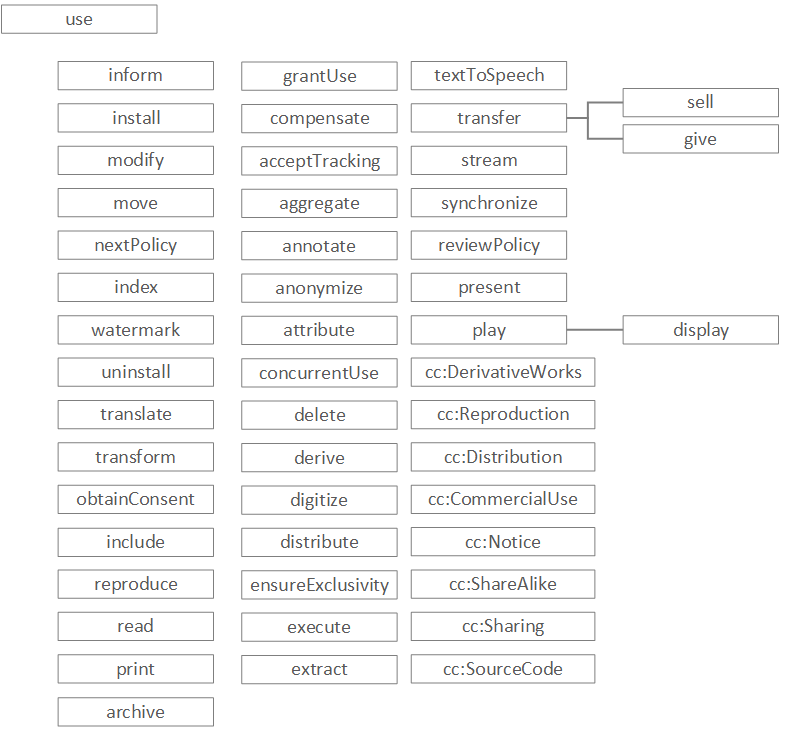
\includegraphics{useTree}}
	
	\caption{Tutte le azioni mostrate sono figlie di use, ad eccezioni di trasfer e le sue sottoazioni\cite{ODRLBestPract}\label{imgUseTransfer}}
\end{figure}


\paragraph{Policy}\mbox{}\\
Come definito nel modello presente nella sezione \ref{modello}, una policy è un gruppo non vuoto di \textbf{regole} e, quindi, di \textbf{permessi}, \textbf{divieti} o \textbf{obblighi}. Una policy deve soddisfare i seguenti requisiti:
\begin{itemize}
	\item deve avere un identificativo univoco, detto \textbf{uid};
	\item deve avere almeno una regola;
	\item può specificare un profilo, obbligatorio se non si usa il Core Vocabulary mostrato nella sezione \ref{profili};
	\item può specificare una policy da cui eredita le proprietà;
	\item può specificare una strategia per la risoluzione dei conflitti.
\end{itemize}
Come visibile dalla figura \ref{ODRLModelSchema}, una policy ha 3 prossibili sottoclassi:
\begin{itemize}
	\item \textbf{Set}: un insieme di regole che hanno effetto;
	\item \textbf{Agreement}: regole concesse ad una entità assegnataria da una assegnatrice;
	\item \textbf{Offer}: proposta di una regola da parte di un assegnatore.
\end{itemize}
Di seguito un esempio di policy definita mediante ODRL:
\begin{lstlisting}[language=json,firstnumber=1,caption={Policy con sottoclasse \textbf{Set}},captionpos=b,label=esmpioPolicy]
{
 "@context": "http://www.w3.org/ns/odrl.jsonld",
 "@type": "Set",
 "uid": "http://example.com/policy:1010",
 "permission": [{
   "target": "http://example.com/asset:9898.movie",
   "action": "use"
 }]
}
\end{lstlisting}
La policy mostrata nel listing \ref{esmpioPolicy} presenta i campi:
\begin{itemize}
	\item @type: serve ad indicarne la sottoclasse;
	\item @context : serve ad indicare che il file deve essere conforme ad ODRL, rappresentato dall'URL da cui si può ottenere l'ODRL Common Vocabulary\cite{ODRLCV};
	\item nel contesto sono presenti altri link per le altre proprietà, ad esempio quello per la descrizione di \textit{Set} e per \textit{use};
	\item non usando termini fuori dai 2 vocabolari principali, non necessita la definizione di un profilo;
	\item l'id univoco è rappresentato da un URL che porta alle informazioni relative la risorsa.
\end{itemize}
\paragraph{Asset}\mbox{}\\
Come definito nel modello presente nella sezione \ref{modello}, un asset è una risorsa o una collezione di risorse soggette a regole. Un asset può essere una qualunque risorsa identificabile. Ha \textbf{AssetCollection} come sottoclasse, la quale rappresenta una collezione di asset. La classe asset può avere:
\begin{itemize}
\item un identificativo univoco, il quale può essere omesso se l'asset è fornito direttamente con la policy; le specifiche di ODRL, pur supportando questo caso d'uso, sconsigliano questa pratica;
\item una o più proprietà denominate \textbf{partOf}: identifica le collezioni di cui fa parte l'asset, il quale può essere a sua volta una collezione.
\end{itemize}
Esempio di utilizzo in una regola:
\begin{lstlisting}[language=json,firstnumber=1,caption={Utilizzo di asset nella proprietà \textbf{target} di una regola},captionpos=b,label=esempioAsset]
{
"@context": "http://www.w3.org/ns/odrl.jsonld",
 "@type": "Offer",
 "uid": "http://example.com/policy:3333",
 "profile": "http://example.com/odrl:profile:02",
 "permission": [{
	"target": "http://example.com/asset:3333",
	"action": "display",
	"assigner": "http://example.com/party:0001"
 }]
}
\end{lstlisting}
La sottoclasse \textbf{AssetCollection} può avere i seguenti 2 campi aggiuntivi:
\begin{itemize}
	\item \textbf{source}: sostituisce il campo \textbf{uid} nelle classe AssetCollection all'interno di un \textbf{refinement};
	\item una o più \textbf{refinement}: limiti riguardanti la collezione che identificano solamente un sottogruppo di asset al suo interno.
\end{itemize}
Esempio di utilizzo della proprietà \textbf{partOf}:
\begin{lstlisting}[language=json,firstnumber=1,caption={L'asset definito è parte del target presente nel listing \ref{esempioAsset}},captionpos=b,label=esempioAssetColl]
{
	"@type": "dc:Document",
	"@id": "http://example.com/asset:111.doc",
	"dc:title": "Annual Report",
	...
	"odrl:partOf": "http://example.com/archive1011",
	...
}
\end{lstlisting}
In quest'ultimo esempio si ha che l'asset con id ``\url{http://example.com/asset:111.doc}'' è definito come parte della collezione ``\url{http://example.com/archive1011}''. Questa definizione ha come effetto l'applicarsi della policy presente nel listing \ref{esempioAsset} anche all'asset che fa parte della collezione.
\paragraph{Party}\mbox{}\\
Come definito nel modello presente nella sezione \ref{modello}, un party è una entità o una collezione di entità con una funzione determinata in una regola. Un party può essere un qualunque soggetto con un ruolo attivo nelle regole o che produce un effetto specifico, ad esempio controlla che le azione relative ad un dovere vengano effettuate. Ha \textbf{PartyCollection} come sottoclasse, la quale rappresenta una collezione di entità. La classe party può avere:
\begin{itemize}
	\item un identificativo univoco, il quale può essere omesso se è possibile definire in altro modo l'entità; le specifiche di ODRL, pur supportando questo caso d'uso, sconsigliano questa pratica;
	\item una o più proprietà denominate \textbf{partOf}: identifica le collezioni di cui fa parte l'entità, la quale può essere a sua volta una collezione.
\end{itemize}
Esempio di utilizzo in una regola:
\begin{lstlisting}[language=json,firstnumber=1,caption={Utilizzo di party nelle proprietà \textbf{assigner} ed \textbf{assignee} di una regola},captionpos=b,label=esempioParty]
{
"@context": "http://www.w3.org/ns/odrl.jsonld",
"@type": "Agreement",
"uid": "http://example.com/policy:8888",
"profile": "http://example.com/odrl:profile:04",
"permission": [{
"target": "http://example.com/music/1999.mp3",
"assigner": "http://example.com/org/sony-music",
"assignee": "http://example.com/people/billie",
"action": "play"
}]
}  
\end{lstlisting}
La sottoclasse \textbf{PartyCollection} può avere i seguenti 2 campi aggiuntivi:
\begin{itemize}
	\item \textbf{source}: sostituisce il campo \textbf{uid} nelle classe PartyCollection all'interno di un \textbf{refinement};
	\item una o più \textbf{refinement}: limiti riguardanti la collezione che identificano solamente un sottogruppo di asset al suo interno.
\end{itemize}
Esempio di utilizzo della proprietà \textbf{partOf}:
\begin{lstlisting}[language=json,firstnumber=1,caption={L'entità definita è parte di una PartyCollection},captionpos=b,label=esempioPartyColl]
{
"@type": "vcard:Individual",
"@id": "http://example.com/person/murphy",
"vcard:fn": "Murphy",
"vcard:hasEmail": "murphy@example.com",
...
"odrl:partOf": "http://example.com/team/A",
...
}
\end{lstlisting}
In quest'ultimo esempio si ha che l'entità con id ``\url{http://example.com/person/murphy}'' è definita come parte della collezione ``\url{http://example.com/team/A}''. Questa definizione ha come effetto l'affidare le funzioni di quest'ultima collezione anche alla singola entità che ne fa parte.
\paragraph{Action}\mbox{}\\
Come definito nel modello presente nella sezione \ref{modello}, \textbf{action} è una classe che rappresenta un'operazione che può essere esercitata su un asset, al quale viene associata mediante la propietà \textbf{action} di una regola. Nell' ODRL Core Vocabulary sono presenti 2 azioni principali:
\begin{itemize}
	\item use: un qualsiasi utilizzo dell'asset;
	\item transfer: una qualsiasi azione che preveda il trasferimento di proprietà dell'asset;
\end{itemize}
Un'azione può avere le seguenti proprietà:
\begin{itemize}\label{includesProp}
	\item refinement: raffinamenti semantici sull'azione, come ad esempio l'ammontare di un pagamento, il luogo nel quale l'azione può essere eseguita o il tempo massimo di esecuzione;
	\item includedIn: esprime l'azione padre; la conseguenza di questa dichiarazione risulta essere che tutte le regole applicate all'azione padre, devono valere anche per l'azione figlia;
	\item implies: esprime un'azione che non deve essere vietata per permettere l'azione con questa proprietà, ma le 2 azioni non hanno una relazione espressa tramite \textit{includedIn}\footnote{attualmente né l'ODRL Core Vocabulary né l'ODRL Common Vocabulary presentano azioni con questa proprietà}. 
\end{itemize}
Come anticipato nel paragrafo \ref{profili} relativo ai profili, l'ORDL Common Vocabulary utilizza la proprietà \textit{includedIn} per aggiungere azioni figlie sia ad \textit{use} che \textit{transfer}, come già mostrato nella figura \ref{imgUseTransfer}.\\
Di seguito un esempio di azione in una regola:
\begin{lstlisting}[language=json,firstnumber=1,caption={L'azione \textbf{play} è presente nella proprietà \textbf{action} della regola},captionpos=b,label=esempioAction]

{
	"@context": "http://www.w3.org/ns/odrl.jsonld",
	"@type": "Offer",
	"uid": "http://example.com/policy:1012",
	"profile": "http://example.com/odrl:profile:06",
	"permission": [{
		"target": "http://example.com/music:1012",
		"assigner": "http://example.com/org:abc",
		"action": "play"
	}]
}
\end{lstlisting}
\paragraph{Constraint e Logical Constraint}\mbox{}\\
Come definito nel modello presente nella sezione \ref{modello}, \textbf{constraint} è una classe usata per comparare 2 espressioni che non sono constraint a loro volta, utilizzando un operatore relazionale. Rappresentano una limitazione tramite un confronto, la quale può essere soddisfatta o non soddisfatta. La classe presenta le seguenti proprietà:
\begin{itemize}
	\item uno o nessun identificativo univoco, qualora si volesse riutilizzare l'espressione di confronto definita;
	\item un \textbf{leftOperand}: elemento a sinistra dell'operatore di confronto;
	\item un sottotitpo \textbf{operator}: operatore di confronto;
	\item uno tra: 
	\begin{itemize}
		\item \textbf{rightOperand}: elemento a destra dell'operatore di confronto, identificato direttamente;
		\item \textbf{rightOperand}: elemento a destra dell'operatore di confronto, identificato con un riferimento; 
	\end{itemize} 
	\item uno o nessun \textbf{dataType}: definisce il tipo dell'operando di destra;
	\item una o nessuna \textbf{unit}: unità di misura dell'operando di destra;
	\item uno o nessun \textbf{status}: per l'elemento di sinistra.
\end{itemize}
Oltre ai normali constraint, il modello definisce anche dei logical constraint, ovvero operazioni logiche su altri constraint già definiti. In questo caso le proprietà sono:
\begin{itemize}
	\item uno o nessun identificativo univoco, qualora si volesse riutilizzare l'espressione di confronto definita;
	\item un sottotipo di \textbf{operand}: operatore logico tra i constraint espressi come lista al suo interno.
\end{itemize}
Esempi di utilizzi dei constraint: 
\begin{lstlisting}[language=json,firstnumber=1,caption={Constraint su azione: l'azione \textbf{print} è permessa solo per risoluzioni minori di 1200 dpi},captionpos=b,label=esempioRef]
{
 "@context": "http://www.w3.org/ns/odrl.jsonld",
 "@type": "Offer",
 "uid": "http://example.com/policy:6161",
 "profile": "http://example.com/odrl:profile:10",
 "permission": [{
  "target": "http://example.com/document:1234",
   "assigner": "http://example.com/org:616",
   "action": [{
  	"rdf:value": { "@id": "odrl:print" },
  	"refinement": [{
  		"leftOperand": "resolution",
  		"operator": "lteq",
  		"rightOperand": { "@value": "1200", "@type": "xsd:integer" },
  		"unit": "http://dbpedia.org/resource/Dots_per_inch"
    	}]
 	}]
  }]
}
\end{lstlisting}
\begin{lstlisting}[language=json,firstnumber=1,caption={Constraint logico su azione: l'azione \textbf{reproduce} è permessa solo nella forma di uno dei due constraint listati},captionpos=b,label=esempioLogRef]
{
 "@context": "http://www.w3.org/ns/odrl.jsonld",
 "@type": "Offer",
 "uid": "http://example.com/policy:88",
 "profile": "http://example.com/odrl:profile:10",
 "permission": [{
  "target": "http://example.com/book/1999",
  "assigner": "http://example.com/org/paisley-park",
  "action": [{
    "rdf:value": { "@id": "odrl:reproduce" },
	"refinement": {
	  "xone": { 
	    "@list": [ 
		 { "@id": "http://example.com/p:88/C1" },
		 { "@id": "http://example.com/p:88/C2" } 
		]}
	}
  }]
 }]
}
\end{lstlisting}
\begin{lstlisting}[language=json,firstnumber=1,caption={Constraint su asset: l'azione \textbf{play} è permessa solo sui target di durata strettamente inferiore a 60 minuti},captionpos=b,label=esempioConAss]
{
"@context": "http://www.w3.org/ns/odrl.jsonld",
"@type": "Offer",
"uid": "http://example.com/policy:4444",
"profile": "http://example.com/odrl:profile:11",
"permission": [{
 "assigner": "http://example.com/org88",
 "target": {
 	"@type": "AssetCollection",
 	"source":  "http://example.com/media-catalogue",
 	"refinement": [{
 		"leftOperand": "runningTime",
 		"operator": "lt",
 		"rightOperand": { 
 		 "@value": "60",
 		 "@type": "xsd:integer"
 		 },
 		"unit": "http://qudt.org/vocab/unit/MinuteTime"
 	}]
 },
 "action": "play"
}]
}
\end{lstlisting}
\begin{lstlisting}[language=json,firstnumber=1,caption={Constraint su party: l'azione \textbf{view} è permessa solo alle entità con età strettamente superiore a 17 anni},captionpos=b,label=esempioConParty]
{
"@context": "http://www.w3.org/ns/odrl.jsonld",
"@type": "Agreement",
"uid": "http://example.com/policy:4444",
"profile": "http://example.com/odrl:profile:12",
"permission": [{
  "target": "http://example.com/myPhotos:BdayParty",
  "assigner": "http://example.com/user44",
  "assignee": {
     "@type": "PartyCollection",
 	 "source":  "http://example.com/user44/friends",
 	 "refinement": [{
 	 	"leftOperand": "foaf:age",
 	 	"operator": "gt",
 	 	"rightOperand": { 
 	 	 "@value": "17",
 	 	 "@type": "xsd:integer"
 		 }
 	 }]
 	},
  "action": { "@id": "ex:view" }
}]
}
\end{lstlisting}
\paragraph{Rule}\label{ODRLRulePara}\mbox{}\\
Come definito nel modello presente nella sezione \ref{modello}, \textbf{rule} è una classe astratta che raccoglie gli aspetti comuni della classi  \textbf{permission}, \textbf{prohibition}, and \textbf{duty}. Rappresenta una delle regole all'interno della policy. Presenta le seguenti proprietà:
\begin{itemize}
	\item una \textbf{action}: azione regolamentata;
	\item una o nessuna \textbf{relation}: asset sul quale si applica la regola;
	\item una, nessuna o più \textbf{function}: funzioni che un party può avere all'interno di una regola;
	\item uno, nessuno o più \textbf{constraint }: limiti applicati alla validità della regola;
	\item uno o nessun identificativo univoco, necessario solo qualora si usare la regola per ereditarne le proprietà;
\end{itemize}
Le sottoclassi sono così definite:
\begin{itemize}
	\item \textbf{permission}: permette un'azione sull'asset specificato, con tutti i \textbf{refinement} di quest'ultima soddisfatti; inoltre l'azione può essere eseguita solo se tutti i limiti della regola sono soddisfatti e ogni dovere espresso come \textbf{duty} è stato rispettato. Un permesso rende obbligatoria la \textbf{relation} denominata \textbf{target};
	\item \textbf{prohibition}: vieta un'azione sull'asset specificato, con tutti i \textbf{refinement} di quest'ultima soddisfatti; inoltre l'azione non può essere eseguita solo se tutti i limiti della regola sono soddisfatti; se si infrange il divieto, ogni dovere espresso come \textbf{remedy} deve essere eseguito. Un divieto rende obbligatoria la \textbf{relation} denominata \textbf{target};
	\item \textbf{duty}: obbligo di eseguire un'azione, con tutti i \textbf{refinement} di quest'ultima soddisfatti; un dovere è compiuto se tutti i suoi limiti sono soddisfatti e la sua azione effettuata, con tutti i \textbf{refinement} definiti. Se un dovere non è stato compiuto, bisogna eseguirne le \textbf{consequences}, ovvero altri doveri da compiere.
\end{itemize}
Esempi di regole all'interno di policy:
\begin{lstlisting}[language=json,firstnumber=1,caption={La regola esprime il permesso di eseguire l'azione \textbf{play} sul target fino al giorno 2017-12-31 compreso},captionpos=b,label=esempioPerm]
{
 "@context": "http://www.w3.org/ns/odrl.jsonld",
 "@type": "Offer",
 "uid": "http://example.com/policy:9090",
 "profile": "http://example.com/odrl:profile:07",
 "permission": [{
    "target": "http://example.com/game:9090",
    "assigner": "http://example.com/org:xyz",
    "action": "play",
    "constraint": [{
        "leftOperand": "dateTime",
        "operator": "lteq",
        "rightOperand": { "@value": "2017-12-31", "@type": "xsd:date" }
    }]
  }]
}
\end{lstlisting}
\begin{lstlisting}[language=json,firstnumber=1,caption={La regola esprime il divieto di eseguire l'azione \textbf{archive} sul target},captionpos=b,label=esempioPro]
{
 "@context": "http://www.w3.org/ns/odrl.jsonld",
 "@type": "Agreement",
 "uid": "http://example.com/policy:5555",
 "profile": "http://example.com/odrl:profile:08",
 "prohibition": [{
	"target": "http://example.com/photoAlbum:55",
	"action": "archive",
	"assigner": "http://example.com/MyPix:55",
	"assignee": "http://example.com/assignee:55"
 }]
}
\end{lstlisting}

\begin{lstlisting}[language=json,firstnumber=1,caption={La regola esprime l'obbligo di eseguire l'azione \textbf{compensate}, specificando come \textbf{refinement} l'ammontare del pagamento},captionpos=b,label=esempioDuty]
{
"@context": "http://www.w3.org/ns/odrl.jsonld",
"@type": "Agreement",
"uid": "http://example.com/policy:42",
"profile": "http://example.com/odrl:profile:09",
"obligation": [{
 "assigner": "http://example.com/org:43",
 "assignee": "http://example.com/person:44",
 "action": [{
   "rdf:value": {
     "@id": "odrl:compensate"
   },
   "refinement": [
     {
     "leftOperand": "payAmount",
     "operator": "eq",
     "rightOperand": { "@value": "500.00", "@type": "xsd:decimal" },
     "unit": "http://dbpedia.org/resource/Euro"
   }]
  }]
 }]
}
\end{lstlisting}
\subsection{Problematica trattata}\label{problematiche}
\paragraph{Gestione dei conflitti}\mbox{}\\
La trattazione fatta fino ad ora per ODRL prende in considerazione la definizione di una singola policy per volta. Questo caso non rispecchia però le necessità reali che il linguaggio punta a soddisfare ed, in particolare, non rispecchia i casi d'uso definiti in MOSAICO, dove è naturale che vi sia un numero molto alto di policy definite.\\
ODRL propone già alcuni elementi per permettere la definizione di più policy in modo agevole, ad esempio: 
\begin{itemize}
	\item è possibile utilizzare la proprietà \textbf{inheritFrom} per permettere ad una policy di ereditare tutte le regole definite in un'altra policy;
	\item è possibile utilizzare la proprietà \textbf{conflict} definire una strategia di risoluzione dei conflitti; le strategia attualmente definite nel modello sono le seguenti:
	\begin{itemize}
		\item \textbf{perm}: le regole di tipo \textbf{permission} hanno la priorità in caso di conflitto;
		\item \textbf{prohibit}: le regole di tipo \textbf{prohibition} hanno la priorità in caso di conflitto;
		\item \textbf{invalid}: in caso di conflitto, la policy risulta non valida nella sua interezza; è il valore di default se non definito esplicitamente.
	\end{itemize}
\end{itemize}
Questo sistema di gestione dei conflitti risulta avere però una problematica fondamentale all'interno dei casi d'uso di MOSAICO: si riferisce a conflitti all'interno di una singola policy o che avvengono in seguito all'utilizzo della proprietà \textbf{inheritFrom}; risulta possibile notare che in uno scenario multi-owner, come quello di MOSAICO, l'utilizzo della proprietà \textbf{conflict} risulta inadatto, ad esempio:
\begin{enumerate}
	\item si supponga che un ospedale, indicato come A, voglia rendere disponibili i propri dati di ricerca in un mercato come quello di MOSAICO;
	\item risulta plausibile che la collezione di dati di questo ospedale venga inserita in una raccolta di referti medici, i cui owner sono vari ospedali situati in stati diversi;
	\item il dato fornito da A viene accompagnato da una policy ODRL, la quale può utilizzare la proprietà \textbf{inheritFrom} per inserire nella propria policy le regole richieste da normative europee;
	\item oltre a questo, A inserisce nella policy anche regole relative a norme sulla privacy vigenti nel proprio paese, settando la proprietà \textbf{conflict} a \textbf{prohibit}, al fine di proteggere i dati sensibili degli utenti trattati dalla propria collezione dati.
\end{enumerate}
Se si considera lo scenario mostrato in esempio non multi-owner, ODRL riesce perfettamente ad soddisfare le esigenze dell'owner della collezione di dati, permettendogli di aderire alle normative europee ed, allo stesso tempo, di tutelare la privacy dei propri pazienti in conformità con le normative vigenti nel suo paese.\\
Nel caso in cui, la collezione di dati medici appartenga a più ospedali, questa soluzione non risulta più adatta, in particolare nel seguente caso:
\begin{enumerate}
	\item un secondo ospedale, indicato come B, segue il medesimo procedimento ma lascia la proprietà \textbf{conflict} uguale ad \textbf{invalid};
	\item se le norme dei paesi di A e B non sono le stesse, entrambe le policy vengono invalidate nella loro totalità, anche se in disaccordo solo su un sottoinsieme di regole;
	\item questo comportamento risulta deleterio sia per quanto concerne il mercato, poiché scoraggia degli owner a partecipare ad una collezione; \item il comportamento mostrato risulta dannoso anche per quanto concerne i soggetti dei dati, non più tutelati da regole poiché invalidate.
\end{enumerate}
Una possibile soluzione a questo problema è attuare il merging delle varie policy che targettano la collezione di dati, rendendo l'azione sulle varie regole più granulare; prendendo ad esempio l'ultimo scenario mostrato:
\begin{enumerate}
	\item avendo due strategie di conflitto differenti, nessuna delle due viene considerata;
	\item per ogni regola in conflitto, si tengono solamente le regole di divieto, seguendo l'obiettivo di MOSAICO di tutela della privacy;
	\item per ogni regola non in conflitto, la regola viene mantenuta, seguendo l'obiettivo d MOSAICO di portare un dato di qualità ed accessibile;
	\item per ogni regola definita come permessa solo in una policy, la si invalida, poiché la seconda policy non si esprime in merito.
\end{enumerate}
Questo procedimento è solo uno dei possibili, in base alle casistiche di conflitto possibili e risulta in linea con i requisiti che MOSAICO punta a soddisfare, poiché a differenza di quanto definito in ODRL:
\begin{itemize}
	\item porta ad una diminuzione della qualità del dato graduale, anziché ad una invalidazione totale della policy al primo conflitto;
	\item durante la diminuzione della qualità del dato, preserva comunque il maggior grado di tutela della privacy che le policy definite possono offrire, poiché permette sempre e solo azioni che hanno una regola esplicita che le riguarda.
\end{itemize}
\paragraph{Controllo inefficiente}\mbox{}\\
Uno dei requisiti fondamentali che MOSAICO punta a soddisfare è l'efficienza. Utilizzando il modello finora espresso, questo requisito viene meno, poiché si è sempre costretti a controllare tutte le regole all'interno di una policy: ciò accade a causa della proprietà \textit{includedIn} di un'azione. Di seguito un esempio della problematica:
\begin{itemize}
\item all'interno di una policy sono presenti le seguenti 2 regole:
\begin{itemize}
\item è permessa l'azione \textbf{transfer};
\item non è permessa l'azione \textbf{sell};
\end{itemize}
\item oltre alle regole espresse, ne sono presenti altre;
\item come visibile nella figura \ref{imgUseTransfer}, l'azione \textbf{transfer} include le azioni \textbf{sell} e \textbf{give}; 
\item un utente desidera eseguire l'azione \textbf{give} sull'asset interessato dalla policy;
\item un eventuale algoritmo di controllo, non può limitarsi a notare che l'azione \textbf{transfer} sia permessa, risulta costretto a controllare anche che \textbf{give} non sia vietato.
\end{itemize}
Una possibile soluzione a questa problematica può essere implementata mediante i seguenti passi:
\begin{enumerate}
\item invalidare i permessi che comprendono al loro interno un'azione proibita;
\item esprimere i divieti mediante i loro permessi complementari.
\end{enumerate}
Nella casistica mostrata, questa soluzione si andrebbe a tradurre come:
\begin{enumerate}
\item il divieto sull'azione \textbf{sell}, poiché presente insieme al permesso su \textbf{transfer}, produce il permesse sull'effettuare \textbf{give};
\item il permesso sull'azione \textbf{transfer} viene rimosso dalla policy.
\end{enumerate}
Come è possibile notare, un eventuale controllo sulle regole prodotte può fermarsi al primo permesso che trova, anziché controllare anche tutti i divieti presenti nella policy.
\chapter{Tecnologie utilizzate}
All'interno di questo capitolo sono trattate le varie tecnologie e paradigmi utilizzati per implementare una soluzione alle problematiche mostrate nella sezione \ref{problematiche}. Tale problematica necessita lo sviluppo di una componente che attui la semantica necessaria al merging di 2 policy e che mostri il risultato in un formato non ambiguo; al fine di realizzare questo componente, è stato necessario effettuare una ricerca per quanto concerne:
\begin{itemize}
	\item tool già sviluppati per il trattamento di policy ODRL;
	\item tool per interrogare un documento ODRL;
	\item tool per realizzare un documento ODRL.
\end{itemize}
\section{Tool già esistenti}
I risultati relativi della ricerca di tool già realizzati hanno portato le seguenti conclusioni:
\begin{itemize}
	\item gran parte dei tool già sviluppati, non lavorano sull'attuale versione di ODRL\footnote{La versione utilizzata durante la stesura del lavoro di tesi è ODRL v2.2 }, come è possibile notare anche dalla pagina del progetto\cite{ODRLPage};
	\item in particolare, gli unici tool documentati ufficialmente sono:
	\begin{itemize}
		\item alcuni valutatori di stato di una regola all'interno di una policy\cite{evalStatus}, attualmente in sviluppo;
		\item un validatore di policy ODRL\cite{validator}, attualmente in sviluppo;
		\item un editor di policy ODRL\cite{editor};
		\item API per la rappresentazione tramite Java di policy ODRL\cite{api}, supporta ODRL 2.0.
	\end{itemize}
\end{itemize}
Risulta possibile notare che le problematiche di merging e rappresentazione non efficiente delle regole non sono affrontate direttamente dai tool sviluppati, i quali tendono invece ad avere un carattere più generale. Sempre grazie allo scouting è possibile quindi dedurre che l'implementazione di un nuovo tool può non reimplementare i seguenti procedimenti:
\begin{itemize}
	\item eventuali documenti di policy presentati in ingresso possono essere validati in precedenza;
	\item non necessita di informazioni sullo stato attuale di asset ed attori coinvolti, in quanto lo stato di questi può essere valutato;
	\item non deve supportare nella creazione della policy l'utente.
\end{itemize}
Le uniche componenti relative ai tool già esistenti che nel lavoro esposto sono state reimplementate risultano essere le API per la rappresentazione di policy ODRL in Java: quelle già esistenti sono relative ad una versione di ODRL non attuale e non forniscono interfacce utili al procedimento di merging di 2 policy. 
\section{Interrogazione e produzione documenti ODRL}
Le ricerche relative al parsing ed alla produzione di un documento ODRL, hanno portato al framework Apache Jena\cite{Jena}, utilizzato per creare applicazioni secondo i modelli  ``Semantic web''\cite{SemanticWeb} e  ``Linked Data''. Il framework ed i modelli di cui supporta la creazione, sono descritti nelle sezioni seguenti.
\subsection{Semantic Web}
Il Semantic Web è definita come un'estensione del World Wide Web, nel quale i dati all'interno della rete \textit{machine-readable}. In particolare ``nel contesto del Semantic Web, il termine semantico assume la valenza di
"elaborabile dalla macchina" e non intende fare riferimento alla semantica del 
linguaggio naturale e alle tecniche di intelligenza artificiale. Il Semantic Web è, come l’
XML, un ambiente dichiarativo, in cui si specifica il significato dei dati, e non il modo
in cui si intende utilizzarli''\cite{introSem}. Alla base dell'idea del Semantic Web vi sono:
\begin{itemize}
	\item le risorse, non necessariamente interpretabili da una macchina;
	\item i metadati connessi alle risorse, i quali sono machine-readable.
\end{itemize}
Per realizzare quest'idea, risulta necessario poter standardizzare i metadati collegati alle risorse, specificandone semantica e sintassi.\\
Il formato sintattico scelto come standard è il modello Resource Description Framework (RDF)\cite{RDF}, mentre invece si lascia libertà sulla semantica, la quale può venir specificata mediante vocabolari relativi al dominio, utilizzando RDF Schema\cite{RDFS}. Sia RDF che RDFS sono descritti in dettaglio nelle prossime sezioni.\\
Prendendo come esempio il listing \ref{esempioAsset}, risulta possibile notare:
\begin{itemize}
	\item il documento ODRL è la rappresentazione machine-readable di un documento di specifica dei requisiti d'accesso ad una risorsa;
	\item la sintassi è standard ed è in formato RDF;
	\item la semantica è stata definita per gli scopi necessari ad ODRL, esplicitandone gli elementi nel \textbf{contesto};
	\item la risorsa alla quale è collegato il metadato non è specificata, ma il metadato dà informazioni utili su tutte le risorse presenti, fornendo un'informazione non centralizzata poiché recuperabile con query relative a varie risorse o semplicemente allegando il metadato a più risorse.
\end{itemize}
\subsection{Linked Data}
Fino ad ora, si è mostrato i principi scelti come base per rendere ogni risorsa machine-readable, permettendo ad una macchina di ottenere maggiori informazioni sulla risorsa.\\
Il Semantic Web non cerca solamente di migliorare la qualità dell'informazione sulla singola risorsa, bensì di fornire ad un applicativo la possibilità di consultare informazioni relative anche a risorse collegate a quella iniziale.\\
Questo secondo obiettivo viene attuato mediante i 4 principi dei Linked Data, già enunciati nella sezione \ref{linkedDataPrinc}.\\
Un importate risultato raggiunto in questo ambito risulta essere DBPedia\cite{dbpedia}, progetto che permette:
\begin{itemize}
	\item di consultare Wikipedia in formato RDF;
	\item collega gli articoli Wikipedia a risorse presenti al di fuori del sito, permettendo così di effettuare query che recuperano informazioni da più fonti. 
\end{itemize}
Come già citato, questo modello è ben visibile all'interno di ODRL, per esempio nel listing \ref{esmpioPolicy} è possibile notare:
\begin{itemize}
	\item che la policy ha un proprio URI, risulta quindi sia un metadato, che una risorsa consultabile a sé;
	\item in quanto risorsa consultabile, ha al suo interno diversi URI relativi ad altre risorse, come ad esempio:
	\begin{itemize}
		\item l'URI relativo all'asset target della policy;
		\item l'URI relativo al contesto del documento, il quale contiene a suo volta informazioni utili per leggere correttamente una policy;
	\end{itemize}
\end{itemize}
\subsection{RDF}
``RDF, o \textit{Resource Description Framework}, si pone alle fondamenta del processing di metadati; fornisce interoperabilità tra applicazioni che si scambiano infromazioni machine-readable nel Web. RDF enfatizza procedure per abilitare l'elaborazione automatica per risorse web''\cite{RDF}. Tra i casi d'uso supportati da RDF vi sono:
\begin{itemize}
\item recupero di risorse web per ottenere migliori motori di ricerca;
\item catalogazione di contenuto ed espressione di relazioni tra varie fonti nel Web;
\item rappresentazione di proprietà intellettuale e diritti relativi ad una risorsa Web.
\end{itemize}
RDF inoltre, condivide la visione per la quale un metadato può essere a sua volta un dato, poiché per all'interno del framework è si definisce come risorsa qualsiasi entità identificabile mediante un URI.\\
Tra le caratteristiche di RDF vi è il proporre una sintassi che per descrivere risorse che sia indipendente dal dominio di applicazione: 
\begin{itemize}
\item non vi sono assunzioni specifiche di dominio applicativo;
\item non vi sono restrizioni di semantica, definibile in base al dominio.
\end{itemize}
La sintassi mostrata, fa riferimento a ciò che è definito come \textit{serialization syntax}: formato XML per la rappresentazione del modello RDF. Tale sintassi non è l'unica possibile né l'unica valida:
\begin{itemize}
\item la \textit{serialization syntax} si riferisce al lavoro che la W3C sta svolgendo in questo ambito per affinare il modello RDF;
\item altre rappresentazioni possono essere più utili in base allo scenario applicativo, per esempio nel caso in cui il documento debba essere anche leggibile da persone.
\end{itemize}
\paragraph{Il modello RDF}\mbox{}\\
Il modello RDF è definito come segue\cite{RDF}:
\begin{enumerate}
\item dato un insieme di nodi, definito come N;
\item sia un sottoinsieme di N, detto \textit{PropertyTypes}, definito come P;
\item sia un insieme di triple, definito come T, i cui elementi vengono informarmalmente chiamati proprietà. Il primo elemento di ogni tripla è un elemento di P, il secondo un elemento di N ed il terzo può essere un elemento di N o un valore atomico, ad esempio una stringa Unicode.
\end{enumerate}
La rappresentazione del modello equivale ad un grafo orientato, i cui nodi sono le risorse descritte o i valori che le descrivono; gli archi che collegano i nodi presentano come label i nomi dei \textit{PropertyTypes} che li collegano. Per esempio:
\begin{enumerate}
\item la frase \\``Ora Lassila" è l' "autore" della pagina web ``http://www.w3.org/People/Lassila''''
\item è serializzata come \\ \{autore, [http://www.w3.org/People/Lassila], "Ora Lassila"\}
\item dalla definizio del modello, è possibile dedurre che la label \textit{autore} è il nome di un nodo appartenente a P;
\item tale nodo, identificato con X,avrà a sua volta le seguenti serializzazioni:
\begin{enumerate}
\item \{PropName,  X, author\}
\item \{PropObj,   X, [http://www.w3.org/People/Lassila]\}
\item \{PropValue, X, "Ora Lassila"\}
\end{enumerate}

\end{enumerate}
Nell'esempio precedente, si è mostrato il tipo di asserzione più semplice che RDF è in grado di supportare; quanto segue mostra come si possano creare relazioni tra le varie risorse:
\begin{enumerate}
\item la frase \\``Ralph crede che il documento 'L'origine delle specie' abbia come autore Charles Darwin''
\item è serializzata come \\ \{crede, "Ralph", Statement1\}
\item le serializzazioni relative al nodo di \textit{crede}, identificato con X, sono:
\begin{enumerate}
\item \{PropName,  X, crede\}
\item \{PropObj,   X, Ralph\}
\item \{PropValue, X, Statement1\}
\end{enumerate}
\item \textit{Statement1} è un elemento di T, ovvero un tripla;
\item le serializzazioni relative a Statement1 sono:
\begin{enumerate}
\item \{PropName, Statement1, autore\}
\item \{PropObj, Statement1, [http://loc.gov/Books/OrigineSpecie]\}
\item \{PropValue, Statement1, Charles Darwin\}
\end{enumerate}
\end{enumerate}
Dagli esempi mostrati, risulta possibile denotare che il cuore del modello RDF siano quindi le triple che si definiscono, dove in ognuna è possibile individuare:
\begin{itemize}
\item \textbf{predicato}: nodo appartente a P;
\item \textbf{oggetto}: nodo sorgente dello statement; appartiene a P ed è il nodo a cui si applica il predicato;
\item \textbf{valore}: nodo destinazione dello statement; appartiene a P, T, o è un valore atomico ed è il valore del predicato.
\end{itemize}
\paragraph{Grammatica RDF e rappresentazione grafica}\mbox{}\\
Il seguente codice mostra un frammento di descrizione di dati conforme al modello RDF tramite XML:
\begin{lstlisting}[language=json,firstnumber=1,caption={Esempio di metadato conforme ad RDF in XML},captionpos=b,label=esempioXML]
<?namespace 
	href="http://docs.r.us.com/bibliography-info"
	as="bib"?> 
<?namespace 
	href="http://www.w3.org/schemas/rdf-schema"
	as="RDF"?> 
<RDF:serialization> 
  <RDF:assertions href="http://www.bar.com/some.doc"> 
    <bib:author>John Smith</bib:author> 
  </RDF:assertions> 
</RDF:serialization>
\end{lstlisting}
Risulta possibile notare i seguenti tag:
\begin{itemize}
\item \textbf{serialization}: indica un insieme di triple all'interno del modello;
\item \textbf{assertions}: indica un'effettiva tripla all'interno del modello, i cui elementi sono individuati nei tag:
\begin{itemize}
\item \textbf{href} nel tag assertions: indica l'oggetto della tripla;
\item \textbf{prefix:PropertyName}: tag definito dall'applicazione che indica il predicato della tripla; il valore di quest elemento XML indica invece il valore del predicato.
\end{itemize}
\end{itemize}
Di seguito la rappresentazione grafica del grafo codificato:
\begin{figure}[H]
\centering
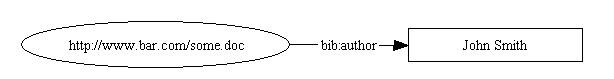
\includegraphics[scale=.50]{../immagini/RDFXML.jpg}
\caption{Rappresentazione grafica del grafo codificato nel listing \ref{esempioXML}}
\label{imgEsempioXML}
\end{figure}
Nell'esempio che segue è invece possibile notare come sfruttare uno statement come valore di una tipla:
\begin{lstlisting}[language=json,firstnumber=1,caption={Esempio di metadato conforme ad RDF in XML},captionpos=b,label=esempioComplexXML]
<?namespace 
  href="http://docs.r.us.com/bibliography-info"
  as="bib"?> 
<?namespace 
  href="http://www.w3.org/schemas/rdf-schema"
  as="RDF"?> 
<RDF:serialization> 
  <RDF:assertions href="http://www.bar.com/some.doc"> 
    <bib:author> 
      <RDF:resource> 
        <bib:name>John Smith</bib:name> 
        <bib:email>john@smith.com</bib:email> 
        <bib:phone>+1 (555) 123-4567</bib:phone> 
      </RDF:resource> 
    </bib:author> 
  </RDF:assertions> 
</RDF:serialization>
\end{lstlisting}
Risulta possibile anche ottenere una scrittura più modulare, sfruttando la proprietà \textit{id} del tag \textit{resource}:
\begin{lstlisting}[language=json,firstnumber=1,caption={Esempio di metadato conforme ad RDF in XML},captionpos=b,label=esempioIdXML]
<?namespace 
	href="http://docs.r.us.com/bibliography-info" 
	as="bib"?> 
<?namespace 
	href="http://www.w3.org/schemas/rdf-schema"
	as="RDF"?> 
<RDF:serialization> 
  <RDF:assertions href="http://www.bar.com/some.doc"> 
    <bib:author href="#John_Smith"/> 
  </RDF:assertions> 
</RDF:serialization>

<RDF:resource id="John_Smith"> 
  <bib:name>John Smith</bib:name> 
  <bib:email>john@smith.com</bib:email> 
  <bib:phone>+1 (555) 123-4567</bib:phone> 
</RDF:resource> 
\end{lstlisting}
Entrambi gli esempi mostrati nei listing \ref{esempioComplexXML} e \ref{esempioIdXML}, si riconducono alla seguente rappresentazione grafica:
\begin{figure}[H]
\centering
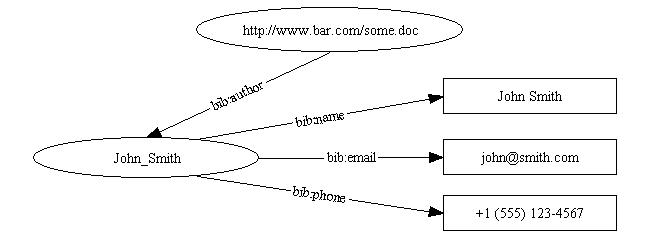
\includegraphics[scale=.50]{/home/oldem/IdeaProjects/actionTree/File documento di tesi/immagini/complexXML.jpg}
\caption{Rappresentazione grafica del grafo codificato nei listing \ref{esempioComplexXML} e \ref{esempioIdXML}}
\label{imgEsempioComplexXML}
\end{figure}
\paragraph{Tag namespace}\mbox{}\\
Il tag \textit{namespace} è un'estensione alla specifica RDF attualmente non mandatorio. Tale tag è stato introdotto per rendere la sintassi relativa alla semantica di un tag specifico di dominio meno prolissa:
\begin{itemize}
 \item \textbf{as}: proprietà del tag che indica il nome del namespace;
 \item \textbf{href}: porzione di identificativo da sostituire alla proprietà \textit{as} quando la si incontra.
\end{itemize} 
Prendendo ad esempio il listing \ref{esempioComplexXML}: il tag \textit{bib:name} è da interpretare come: \\\url{http://docs.r.us.com/bibliography-info/name}\\ quest'ultimo risulta infatti essere l'URI che identifica la proprietà, inoltre è un riferimento a dove è possibile recuperare informazioni su di essa.\\
Il suo utilizzo è denotabile all'interno di ODRL, come ad esempio nel listing \ref{esempioParty}, dove il tag \textit{@context} svolge un ruolo simile: fa riferimento ad un file RDF all'interno del quale sono definite tutte le abbreviazioni utili ad ODRL tramite le seguenti linee di codice:
\begin{lstlisting}[language=json,firstnumber=1,caption={Estratto context ODRL\cite{ODRLContext}},captionpos=b,label=contextJSONLD]
"odrl":       "http://www.w3.org/ns/odrl/2/",
"Permission": "odrl:Permission",
"permission": {"@type": "@id", "@id": "odrl:permission"}
\end{lstlisting}
Come è possibile notare, il formato di serializzazione utilizzato nel listing \ref{contextJSONLD} non è XML, bensì JSON-LD, così come anche nei vari listing presentati nel capitolo \ref{ODRLChapter} relativo ad ODRL.\\
All'interno del lavoro di tesi, le serializzazioni utilizzate sono:
\begin{itemize}
\item JSON-LD: utilizzato negli esempi ed in input al processo di merging;
\item Turtle\cite{Turtle}: utilizzato come output del processo di merging, tale decisione è stata presa poiché risulta essere la serializzazione più matura nel framework Jena.
\end{itemize}
\subsection{RDFS}
Come esposto in precedenza, il modello RDF fornisce la sintassi necessaria per creare metadati in grado di rappresentare relazioni tra le varie risorse, lasciando libertà assoluta sul significato che queste relazioni possono avere. RDFS è ``un'estensione semantica''\cite{RDFS} di RDF che permette di descrivere gruppi di risorse correlate e le relazioni tra le varie risorse. RDFS basa il suo funzionamento sulla definizione di 2 termini:
\begin{itemize}
\item \textbf{rdfs:Class}: raggruppamento di risorse con le stesse proprietà, come ad esempio la classe \textit{odrl:Policy};
\item \textbf{rdf:Property}: relazione tra risorse soggetto e risorse soggetto; istanze di questa particolare classe possiedono, a loro volta, le seguenti proprietà:
\begin{itemize}
\item \textbf{rdfs:range}: i \textit{valori} in una tripla della proprietà devono essere istanze delle classi specificate in questa proprietà;  
\item \textbf{rdfs:domain}: gli \textit{oggetti} in una tripla della proprietà devono essere istanze delle classi specificate in questa proprietà; 
\end{itemize}
\end{itemize}
Oltre a quanto appena mostrato, esistono anche 2 proprietà denominate: \textbf{rdfs:subClassOf} e \textbf{rdfs:subPropertyOf}, le quali permettono di definire un sistema di ereditarietà tra classi e tra proprietà, come ad esempio nel vocabolario ODRL si ha:\\
\begin{lstlisting}[language=json,firstnumber=1,caption={Estratto vocabolario ODRL\cite{ODRVocab}},captionpos=b,label=vocabExtract]
<rdfs:Class 
  rdf:about="http://www.w3.org/ns/odrl/2/Prohibition">
  
  <rdfs:isDefinedBy 
    rdf:resource="http://www.w3.org/ns/odrl/2/"/>
  
  <rdfs:label xml:lang="en">Prohibition</rdfs:label>
  <rdfs:subClassOf
   rdf:resource="http://www.w3.org/ns/odrl/2/Rule"/>
  
</rdfs:Class>
  \end{lstlisting}
L'estratto mostrato è la definizione della sottoclasse \textit{Prohibition}, esposta nella sezione \ref{ODRLRulePara}. Un secondo esempio, sempre visibile in ODRL, è la definizione della proprietà ``odrl:partOf'', mostrata nei listing \ref{esempioAssetColl} e \ref{esempioPartyColl}, tale proprietà:
\begin{itemize}
\item 2 possibili \textit{rdfs:domain} e 2 possibili \textit{rdfs:range};
\item solo 2 coppie \textit{rdfs:domain}-\textit{rdfs:range} sono valide, tale restrizione è espressa mediante OWL\cite{OWL}, ulteriore estensione semantica utilizzata per espriremere concetti logici complessi;
\item all'interno delle proprietà sono specificate le 2 classi \textit{odrl:Party} ed \textit{odrl:Asset}.
\end{itemize}
\subsection{Apache Jena}
``Apache Jena (o Jena) è un framework Java free ed open source per creare applicazioni del semantic web o che sfruttano Linked Data. Il framework è composta da diverse API che interagiscono al fine di processare dati RDF.''\cite{Jena}\\
Per questo motivo si è scelto Jena come insieme di utility sia a supporto della porzione di parsing, descritta nella sezione \ref{parsingSection}, sia a supporto della porzione di produzione del documento ODRL finale, descritta nella sezione \ref{produceSection}. Nel dettaglio, le API utilizzate comprendono:
\begin{itemize}
\item \textbf{Core RDF API};
\item \textbf{Jena schemagen};
\item \textbf{ARQ - A SPARQL Processor for Jena};
\item \textbf{Modulo I/O}.
\end{itemize}
\paragraph{Core RDF API}\mbox{}\\
Questa porzione del framework offre interfacce per l'interazione con il modello RDF. La rappresentazione offerta da questa libreria si basa su triple, i cui elementi sono denominati:
\begin{itemize}
\item \textbf{resource}: l'oggetto dello statement codificato dalla tripla;
\item \textbf{property}: il predicato dello statement;
\item \textbf{value}: il valore dello statement, il quale può essere a sua volta una risorsa.
\end{itemize}
L'interfaccia core fornita da questo componente è denominata \textit{Model}, il quale denota un'intero grafo RDF; questa interfaccia è intesa per supportare operazioni molto astratte sull'intero modello, e può essere usata per:
\begin{itemize}
\item specificare su quale file o collezione di file RDF si sta lavorando;
\item aggiungere, recuperare e rimuovere nodi dal grafo;
\item settare i \textit{namespace} utilizzati all'interno del modello;
\item settare la serializzazione con la quale il modello viene mostrato;
\item interagire con l'API ARQ per l'interrogazione del modello tramite query SPARQL.
\end{itemize}
\paragraph{Jena schemagen}\mbox{}\\
Questo tool fornito dal framework ha utilità puramente tecnica, in quanto è uno strumento per ``convertire vocabolari OWL o RDFS in una classe Java class che contiene costanti statiche per i termini nel vocabolario''.\\
L'effettivo utilizzo del tool si traduce nel suo processare un file RDF, in questo caso il file context di ODRL\cite{ODRLContext}, automatizzando il processo di estrazione dei termini all'interno del vocabolario. I vantaggi di questo approccio si traducono in:
\begin{itemize}
\item l'utilizzo di variabili facilmente leggibili all'interno del linguaggio ARQ, anziché dell'URI che definisce la classe o la proprietà;
\item interazione più trasparente con le \textit{Core RDF API} in fase di aggiunta risorse o di definizione delle proprietà di un nodo.
\end{itemize}
Il contributo di questo tool non è direttamente visibile all'interno del codice del progetto di tesi, poiché è stata sfruttata la versione standalone del tool.
\paragraph{ARQ e SPARQL}\mbox{}\\
``ARQ è il query engine fornito da Jena che supporta il linguaggio SPARQL RDF Query.''\cite{Jena}\\
Il linguaggio ``SPARQL può essere usato per esprimere query su diverse sorgenti di dati, sia su dati nativi RDF o esposti come RDF via middleware.''\cite{SPARQL}\\
L'obiettivo di queste tecnologie è fornire interfacce che permettano l'interrogazione di modelli RDF. ARQ è l'API esposta da Jena per formulare tramite Java le interrogazioni; SPARQL è l'effettivo linguaggio nel quale è espressa la query.\\
Prendendo ad esempio il seguente file in formato RDF:\\

\begin{lstlisting}[language=json,firstnumber=1,caption={File sul quale si vuole eseguire una query},captionpos=b,label=SPARQLRDF]
@prefix dc:   <http://purl.org/dc/elements/1.1/> .
@prefix :     <http://example.org/book/> .
@prefix ns:   <http://example.org/ns#> .

:book1  dc:title  "SPARQL Tutorial" .
:book1  ns:price  42 .
:book2  dc:title  "The Semantic Web" .
:book2  ns:price  23 .

\end{lstlisting}
\begin{lstlisting}[language=json,firstnumber=1,caption={Query SPARQL per il recupero dei titoli che iniziano per SPARQL},captionpos=b,label=SPARQLQuery]

PREFIX  dc:  <http://purl.org/dc/elements/1.1/>
SELECT  ?title
WHERE   { ?x dc:title ?title
          FILTER regex(?title, "^SPARQL") 
        }
\end{lstlisting}\mbox{}\\ \\  
Il risultato della query nel listing \ref{SPARQLQuery} è la tupla:
\begin{center} (\textbf{title} = ``SPARQL Tutorial'')\end{center}
Questo secondo esempio mostra come sia possibile filtrare uno statement sulla base di più espressioni:\\
\begin{lstlisting}[language=json,firstnumber=1,caption={File sul quale si vuole eseguire una query},captionpos=b,label=SPARQLRDF2]
@prefix foaf:  <http://xmlns.com/foaf/0.1/> .

_:a  foaf:name   "Johnny Lee Outlaw" .
_:a  foaf:mbox   <mailto:jlow@example.com> .
_:b  foaf:name   "Peter Goodguy" .
_:b  foaf:mbox   <mailto:peter@example.org> .
_:c  foaf:mbox   <mailto:carol@example.org> .
\end{lstlisting}\mbox{}

\begin{lstlisting}[language=json,firstnumber=1,caption={Query SPARQL per il recupero dei nomi e delle mail solo per soggetti che presentano entrambe le proprietà},captionpos=b,label=SPARQLQuery2]
PREFIX foaf:   <http://xmlns.com/foaf/0.1/>
SELECT ?name ?mbox
WHERE
  { ?x foaf:name ?name .
    ?x foaf:mbox ?mbox }
\end{lstlisting}\mbox{}
Il risultato della query nel listing \ref{SPARQLQuery} sono le tuple:
\begin{center}
(\textbf{name} = "Johnny Lee Outlaw", \textbf{mbox} = <mailto:jlow@example.com>)\\
(\textbf{name} = "Peter Goodguy",	\textbf{mbox} = <mailto:peter@example.org>)
\end{center}
Risulta possibile notare che l'ultima tripla presente nel listing \ref{SPARQLRDF2} non sia stata utilizzata per costruire il risultato della query, poiché l'oggetto \textit{\_:c} non ha la proprietà \textit{foaf:mbox}.\\
Il ruolo che hanno le API ARQ all'interno di del progetto è di collegamente tra le query e le \textit{CORE RDF API}, nonché di semplificazione della sintassi, evitando il costrutto \textit{PREFIX} laddove già presente all'interno del modello sul quale si eseguono le query.
\paragraph{Modulo I/O}\mbox{}\\
Il modulo Input/Output fornisce le interfacce necessarie:
\begin{itemize}
\item alla lettura di un file in formato RDF, supportando le serializzazioni:
\begin{itemize}
\item Turtle;
\item N-Triples;
\item N-Quads;
\item TriG;
\item RDF/XML;
\item JSON-LD;
\item RDF/JSON;
\item TriX;
\item RDF Binary;
\end{itemize}
\item alla scrittura di un file in formato RDF, supportando le medesime serializzazione mostrate in lettura.
\end{itemize}
Il modello espresso mediante \textit{CORE RDF API} otttenuto da questi moduli è il medesimo a discapito della serializzazione utilizzata, di conseguenza non è necessario, almeno in lettura, attuare implementazioni specifiche basate sul formato. Quest'ultima constatazione vale anche per il procedimento di parsing e, quindi, per l'intera procedura di merging a valle. L'unica porzione del progetto che necessita di adattamenti in base al formato risulta essere il produttore di documenti ODRL, in quanto alcuni formati possono necessitare di alcuni adattamenti per essere resi più leggibili dagli utenti. Non sono invece necessari adattamenti per l'utilizzo da parte di un programma.
\chapter{Valutazione casistiche}
\section{Casistiche di merging}
\paragraph{Casi base}\mbox{}\\
\subparagraph{Asset diffrenti}\mbox{}\\

\begin{lstlisting}[language=json,firstnumber=1,caption={La policy 1010 permette di riprodurre l'asset 9898.movie a chiunque},captionpos=b]
{
"@context": "http://www.w3.org/ns/odrl.jsonld",
"@type": "Set",
"uid": "http://example.com/policy:1010",
"permission": [{
"target": "http://example.com/asset:9898.movie",
"action": "play"
}]
}

\end{lstlisting}


\begin{lstlisting}[language=json,firstnumber=1,caption={La policy 1011 consente la riproduzione dell'asset 1349.mp3 a chiunque},captionpos=b]
{
"@context": "http://www.w3.org/ns/odrl.jsonld",
"@type": "Set",
"uid": "http://example.com/policy:1011",
"permission": [{
"target": "http://example.com/asset:1349.mp3",
"action": "play"
}]
}
\end{lstlisting}
Le due policy mostrate si riferiscono ad asset differenti, farne il merging porta semplicemente ad una policy avente entrambe le \textit{permission} già enunciate.
\subparagraph{Rule incompatibili}\mbox{}\\
\begin{lstlisting}[language=json,firstnumber=1,caption={La policy 1010 consente la riproduzione dell'asset 9898.movie a chiunque},captionpos=b]
{
"@context": "http://www.w3.org/ns/odrl.jsonld",
"@type": "Set",
"uid": "http://example.com/policy:1010",
"permission": [{
"target": "http://example.com/asset:9898.movie",
"action": "play"
}]
}
\end{lstlisting}
\begin{lstlisting}[language=json,firstnumber=1,caption={La policy 1011 proibisce la distribuzione dell'asset 9898.movie a chiunque},captionpos=b]
{
"@context": "http://www.w3.org/ns/odrl.jsonld",
"@type": "Set",
"uid": "http://example.com/policy:1011",
"prohibition": [{
"target": "http://example.com/asset:9898.movie",
"action": "distribute"
}]
}
\end{lstlisting}
Nonostante le due policy si riferiscano allo stesso asset, anche in questo caso, non è possibile combinare le due regole, poiché si riferiscono a domini diversi. Un eventuale merging delle due policy avrebbe 2 regole distinte uguali a quelle di partenza.\newpage
\subparagraph{Attori designati differenti}\mbox{}\\
\begin{lstlisting}[language=json,firstnumber=1,caption={La policy 0001 permette un qualsiasi utilizzo dell'asset 1212 da parte del soggetto Billie},captionpos=b]
{
"@context": "http://www.w3.org/ns/odrl.jsonld",
"@type": "Policy",
"uid": "http://example.com/policy:0001",
"permission": [{
	"target": "http://example.com/asset:1212",
	"action": "use",
	"assigner": "http://example.com/owner:181",
	"assignee": 
	   "http://example.com/party:person:billie"
}]
}
\end{lstlisting}
\begin{lstlisting}[language=json,firstnumber=1,caption={La policy 0002 proibisce la riproduzione dell'asset 1212 da parte del soggetto Alice},captionpos=b]
{
"@context": "http://www.w3.org/ns/odrl.jsonld",
"@type": "Policy",
"uid": "http://example.com/policy:0002",
"prohibition": [{
"target": "http://example.com/asset:1212",
"action": "play",
"assigner": "http://example.com/owner:181",
"assignee": 
"http://example.com/party:person:alice"
}]
}
\end{lstlisting}
In questo caso, le regole espresse dalle 2 policy sarebbero in conflitto, poiché ``use'', permesso dalla prima policy, comprende al suo interno anche ``play''\footnote{Per le dipendenze tra le azioni, si fa riferimento all'ODRL Core Vocabulary}, proibito dalla seconda. Siccome però le due regole riguardano due soggetti diversi,un eventuale merging delle policy avrebbe 2 regole distinte uguali a quelle di partenza.
\paragraph{Conflitti senza strategia risolutiva indicata}\label{noStrat}\mbox{}\\
Nel caso si presentino 2 policy in conflitto, se non viene indicato alcun processo di risoluzione dei conflitti, secondo lo standard ODRL entrambe le policy sono da considerarsi non valide. Attuando policy merging è possibile formulare una terza policy che racchiude entrambe le casistiche.
\subparagraph{Conflitti permesso-permesso}\label{permperm}\mbox{}\\
\begin{lstlisting}[language=json,firstnumber=1,caption={La policy 0001 permette un qualsiasi utilizzo dell'asset 1212 a chiunque},captionpos=b]
{
"@context": "http://www.w3.org/ns/odrl.jsonld",
"@type": "Policy",
"uid": "http://example.com/policy:0001",
"permission": [{
"target": "http://example.com/asset:1212",
"action": "play"
}]
}
\end{lstlisting}
\begin{lstlisting}[language=json,firstnumber=1,caption={La policy 0002 permette la riproduzione dell'asset 1212 a chiunque},captionpos=b]
{
"@context": "http://www.w3.org/ns/odrl.jsonld",
"@type": "Policy",
"uid": "http://example.com/policy:0002",
"permission": [{
"target": "http://example.com/asset:1212",
"action": "display"
}]
}
\end{lstlisting}
La seconda policy risulta in conflitto con la prima, poiché quest'ultima permette un numero maggiore di utilizzi. Seguendo la procedura standard, entrambe le 2 policy dovrebbero essere considerate invalidate. Nella realtà dei fatti, facendo policy merging, si otterrebbe solamente la policy più restrittiva, ovvero la seconda. La procedura di policy merging in questione sarebbe quindi: 
\begin{enumerate}
	\item invalidare le policy 0001 e 0002;
	\item creare una terza policy 0003, uguale alla 0002(la più restrittiva delle due), con indicato il procedimento di merging;
	\item l'indicazione è opportuna per fare il processo inverso al merging qualora una delle 2 policy originarie venga ritirata.
\end{enumerate}
\subparagraph{Conflitti divieto-divieto}\label{divdiv}\mbox{}\\
\begin{lstlisting}[language=json,firstnumber=1,caption={La policy 0001 proibisce un qualsiasi utilizzo dell'asset 1212 a chiunque},captionpos=b]
{
"@context": "http://www.w3.org/ns/odrl.jsonld",
"@type": "Policy",
"uid": "http://example.com/policy:0001",
"prohibition": [{
"target": "http://example.com/asset:1212",
"action": "play"
}]
}
\end{lstlisting}
\begin{lstlisting}[language=json,firstnumber=1,caption={La policy 0002 proibisce la riproduzione dell'asset 1212 a chiunque},captionpos=b]
{
"@context": "http://www.w3.org/ns/odrl.jsonld",
"@type": "Policy",
"uid": "http://example.com/policy:0002",
"prohibition": [{
"target": "http://example.com/asset:1212",
"action": "display"
}]
}
\end{lstlisting}
Caso duale del precedente; in questo caso una delle due policy proibisce un numero maggiore di utilizzi rispetto all'altra. La procedura da seguire risulta essere:
\begin{enumerate}
	\item invalidare le policy 0001 e 0002;
	\item creare una terza policy 0003, uguale alla 0001(la più ampia delle due), con indicato il procedimento di merging;
	\item l'indicazione è opportuna per fare il processo inverso al merging qualora una delle 2 policy originarie venga ritirata.
\end{enumerate}
\subparagraph{Conflitti permesso-divieto}\label{permdiv}\mbox{}\\
\begin{lstlisting}[language=json,firstnumber=1,caption={La policy 0001 permette il trasferimento dell'asset 1212 al soggetto Alice},captionpos=b]
{
"@context": "http://www.w3.org/ns/odrl.jsonld",
"@type": "Policy",
"uid": "http://example.com/policy:0001",
"permission": [{
"target": "http://example.com/asset:1212",
"assigner": "http://example.com/owner:181",
"assignee": 
"http://example.com/party:person:alice",
"action": "transfer"
}]
}
\end{lstlisting}
\begin{lstlisting}[language=json,firstnumber=1,caption={La policy 0002 proibisce la vendita dell'asset 1212 al soggetto Alice},captionpos=b]
{
"@context": "http://www.w3.org/ns/odrl.jsonld",
"@type": "Policy",
"uid": "http://example.com/policy:0002",
"prohibition": [{
"target": "http://example.com/asset:1212",
"assigner": "http://example.com/owner:181",
"assignee": 
"http://example.com/party:person:alice",
"action": "sell"
}]
}
\end{lstlisting}
In questo caso, l'azione ``transfer'', nell'ODRL Core Vocabulary, è inclusa in 2 sotto-azioni: ``give'' e ``sell''; delle 2 sotto-azioni, solamente ``sell'' è esplicitamente proibita dalla policy 0002, di conseguenza la seguente policy permette solo azioni che soddisfano entrambe le policy precedenti:\newpage
\begin{lstlisting}[language=json,firstnumber=1,caption={La policy 0003 consente al soggetto Alice di cedere l'asset 1212 senza richiedere un compenso e cancellando l'asset dal proprio insieme di dati},captionpos=b]
{
"@context": "http://www.w3.org/ns/odrl.jsonld",
"@type": "Policy",
"uid": "http://example.com/policy:0002",
"permission": [{
"target": "http://example.com/asset:1212",
"assigner": "http://example.com/owner:181",
"assignee": 
"http://example.com/party:person:alice",
"action": "give"
}]
}
\end{lstlisting}
Sono necessarie alcune valutazioni su questa casistica:
\begin{itemize}
	\item il numero di regole all'interno della policy ottenuta per merging non è necessariamente minore rispetto al numero di regole di partenza; tale numero, dipende dal numero di sotto-azioni esistenti e da come è formulato il divieto di partenza;
	\item è necessario un meccanismo per notificare che il le sotto-azioni presentate in realtà indicano ``tutte le sotto-azioni possibili, escluse quelle esplicitamente vietate'';
	\item se ``prohibition'' e ``permission'' fossero invertite tra la policy 0001 e la 0002, la policy 0003 risulterebbe una policy non valida.
\end{itemize}
\paragraph{Conflitti con strategia risolutiva indicata}\mbox{}\\
Le strategie risolutive indicabili all'interno di ODRL utilizzando il Core Vocabulary sono le seguenti:
\begin{enumerate}
	\item ``perm'': tutte le ``permission'' hanno la precedenza sulle ``prohibition'';
	\item ``prohibit'': tutte le ``prohibition'' hanno la precedenza sulle ``permission'';
	\item ``invalid'': qualsiasi conflitto invalida la policy;
\end{enumerate}
La casistica ``invalid'' è già stata trattata all'interno del paragrafo ``Conflitti senza strategia risolutiva indicata''[\ref{noStrat}].\newpage
\subparagraph{Strategia concorde}\mbox{}\\
\begin{lstlisting}[language=json,firstnumber=1,caption={La policy 0001 consente qualsiasi utilizzo dell'asset 1212 a chiunque, dando precedenza ai permessi in caso di conflitto},captionpos=b]
{
"@context": "http://www.w3.org/ns/odrl.jsonld",
"@type": "Policy",
"uid": "http://example.com/policy:0001",
"conflict":{"@type": "perm"},
"permission": [{
"target": "http://example.com/asset:1212",
"action": "use",
"assigner": "http://example.com/owner:181"
}]
}
\end{lstlisting}
\begin{lstlisting}[language=json,firstnumber=1,caption={La policy 0002 permette la riproduzione dell'asset 1212 a chiunque, mentre ne vieta la proiezione, dando precedenza ai permessi in caso di conflitto},captionpos=b]
{
"@context": "http://www.w3.org/ns/odrl.jsonld",
"@type": "Policy",
"uid": "http://example.com/policy:0001",
"conflict":{"@type": "perm"},
"permission": [{
"target": "http://example.com/asset:1212",
"action": "play",
"assigner": "http://example.com/owner:182"
}],
"prohibition": [{
"target": "http://example.com/asset:1212",
"action": "display",
"assigner": "http://example.com/owner:181"
}]
}
\end{lstlisting}
In questo caso è possibile ricondursi alla procedura indicata nel sottoparagrafo ``Conflitti permesso-permesso''[\ref{permperm}] ignorando tutti i divieti espressi nelle policy. In seguito al merging delle policy si ottiene:
\begin{lstlisting}[language=json,firstnumber=1,caption={La policy 0003 risulta essere uguale ai permessi della policy 0002, più restrittiva},captionpos=b]
{
"@context": "http://www.w3.org/ns/odrl.jsonld",
"@type": "Policy",
"uid": "http://example.com/policy:0001",
"conflict":{"@type": "perm"},
"permission": [{
"target": "http://example.com/asset:1212",
"action": "play",
"assigner": "http://example.com/owner:182"
}]
}
\end{lstlisting}
Dando la precedenza ai permessi, rimane comunque da tener in conto che nella policy 0002 il permesso è più ristretto rispetto a quello espresso nella policy 0001.\\
Dualmente, nel caso di strategia di conflitto concorde di tipo ``prohibit'', ci si riconduce al caso mostrato nel sottoparagrafo ``Conflitti divieto-divieto''[\ref{divdiv}], tenendo conto solo dei divieti.
\subparagraph{Strategia discorde}\mbox{}\\
Utilizzando il normale sistema di ereditarietà delle policy di ODRL, una policy contenente 2 strategie di risoluzione dei conflitti dovrebbe essere considerata non valida. Questa casistica si può però ridurre al caso mostrato nel sottoparagrafo ``Conflitti permesso-divieto'' [\ref{permdiv}]. In questo modo, entrambe le policy risultano rispettate. Un'aggiunta che può essere fatta a questa casistica, rispetto a quella già mostrata, sarebbe considerare solamente i divieti o i permessi della singola policy, in base alla strategia indicata; quest'ultima opzione porterebbe ad un ibrido tra le due soluzioni precedenti.
\paragraph{Restrizioni su regole, asset, party}\mbox{}\\
Possono essere poste delle restrizioni sulla validità di una regola o sulla composizione di una collezione di asset o gruppo di soggetti. Anche queste restrizioni possono essere composte similarmente alle regole a sé stanti.\newpage
\begin{lstlisting}[language=json,firstnumber=1,caption={Esempio di limite temporale per una regola, può essere composto similarmente ai limiti sull'azione regolata},captionpos=b]
{
"@context": "http://www.w3.org/ns/odrl.jsonld",
"@type": "Offer",
"uid": "http://example.com/policy:6163",
"profile": "http://example.com/odrl:profile:10",
"permission": [{
	"target": "http://example.com/document:1234",
	"assigner": "http://example.com/org:616",
	"action": "distribute",
	"constraint": [{
		"leftOperand": "dateTime",
		"operator": "lt",
		"rightOperand": 
		  { "@value": "2018-01-01",
		    "@type": "xsd:date" }
		}]
	}]
}
\end{lstlisting}
Problematiche relative alla gestione di questo tipo di merging, non più necessariamente relativo a conflitti, possono essere rilevate nella grande varietà che può assumere:
\begin{itemize}
	\item limiti di tipo temporale;
	\item limiti di tipo spaziale;
	\item limiti di tipo quantitativo(numero di volte che un permesso può essere sfruttato);
	\item limiti relativi al tipo di dato trattato(dimensione dell'immagine, durata del video).
\end{itemize}
A causa di questa varietà, la gestione di questo tipo di merging può facilmente esplodere. Vi è anche da contare che un ``constraint'' può essere ottenuto come operazione in logica booleana di altri ``constraint''. Questo tipo di merging non va necessariamente a risolvere conflitti nelle policy, ma può rilevare quando un numero eccessivo di constraint va a rendere la collezione di asset inutilizzabile(una policy permette l'uso di un asset solo la mattina, la seconda solo la sera, unendole l'asset risulta inutilizzabile).

\chapter{Implementazioni}
\section{Architettura generale}
\begin{figure}[htp]
\centering
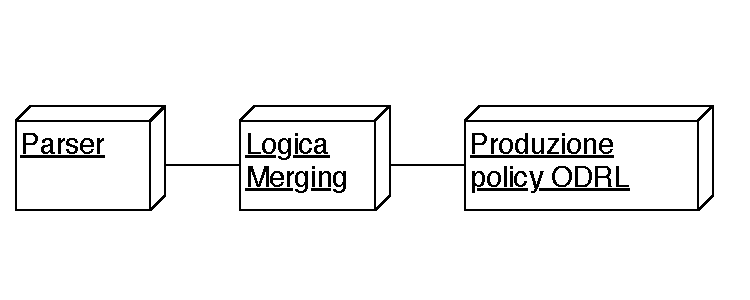
\includegraphics[scale=1]{../immagini/arch_gen.pdf}
\caption{Pipeline dei macro componenti della soluzione}
\label{archGenImpl}
\end{figure}
Come mostrato nella figura \ref{archGenImpl}, l'architettura generale è una semplice pipeline di componenti, poiché l'obiettivo finale risulta attuare trasformazioni sui documenti ODRL in ingresso, per ottenere in uscita un unico documento ODRL che sia:
\begin{itemize}
\item il risultato dell'unione o dell'intersezione delle 2 policy in ingresso;
\item esprima ogni divieto come il suo permesso complementare più ampio.
\end{itemize}
Queste 2 operazioni sono attuate all'interno del componente denominato \textbf{``Logica Merging''}, il quale si occupa di aggiungere la semantica necessaria alle policy ODRL, per poi produrre il documento finale.\\
Il primo componente della pipeline si occupa invece di estrarre le informazioni di rilievo dalle policy in ingresso, mentre il componente in coda si occupa di produrre un documento conforme ad ODRL per dare una forma al risultato ottenuto.
\section{Parser}\label{parsingSection}
//TODO: l'implementazione è iniziata, devo ancora scrivere
\section{Logica Merging}
All'interno di questo componente, è presente la porzione di soluzione atta ad eseguire le effettive operazioni di merging delle policy in ingresso.\\
Le operazioni di merging che si punta a supportare sono di 2 tipi:
\begin{itemize}
\item \textbf{unione}: utilizzata all'iterno di uno scenario collaborativo, i permessi espressi da una sola delle due policy rimangono validi anche all'interno della policy in output;
\item \textbf{intersezione}: utilizzata in uno scenario conservativo, un permesso appare nella policy in output solo se espresso da entrambe le policy in ingresso.
\end{itemize}
\subsection{Rappresentazione delle Azioni}\label{enumAction}
Tra i due focus dell'implementazione vi sono le \textbf{Action}, ovvero gli utilizzi dell'asset regolati dalle policy ODRL. Per rappresentarle, si è utilizzato un enumerativo con la struttura mostrata in figura \ref{imgActionEnum}:
\begin{figure}[H]
\centering
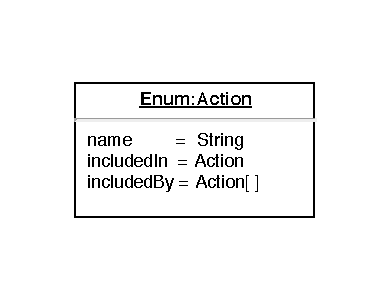
\includegraphics[scale=1.00]{../immagini/enumAction}
\caption{Struttura dell'enumerativo Action}
\label{imgActionEnum}
\end{figure}
All'interno dell'enumerativo è presente il nome che ha all'interno dell' ODRL Common Vocabulary, la lista delle azioni figlio e, se presente, l'azione padre. Tale struttura è assimilabile a quella di un nodo in una struttura dati al albero. L'enumerativo è provvisto dei vari \textit{getter} per il recupero delle informazioni citate.
\subsection{Rappresentazione delle Regole}\label{ruleRappr}
Il secondo focus principale dell'implementazione sono le \textbf{Rule}, il cui stato all'interno della policy è gestito mediante un albero di regole, sfruttando le relazioni che si creano tra le azioni mediante l'enumerativo definito in figura \ref{imgActionEnum}. Per ottenere un maggior incapsulamente delle funzioni, si è deciso di dividere la logica della struttura ad albero in due compenenti, mostrate in figura \ref{imgCompRule} ed esposte di seguito:
\begin{itemize}
\item gestore dell'albero delle regole: questa componente si occupa delle azioni più generali relative l'albero delle regole, come ad esempio il recupero di un nodo specifico, il settaggio di stato di un nodo, oppure il recupero dello stato di ogni regola;
\item gestore del singolo nodo: questo nodo si occupa dell'effetiva gestione del nodo rappresentante una regola relativa ad un'azione, di conseguenza attua operazioni come il recupero del nodo padre o dei nodi figli; le funzioni principali riguardano però la propagazione di eventuali divieti lungo la gerarchia delle regole, sia verso i nodi figli che verso il nodo padre.
\end{itemize}

\begin{figure}[H]
\centering
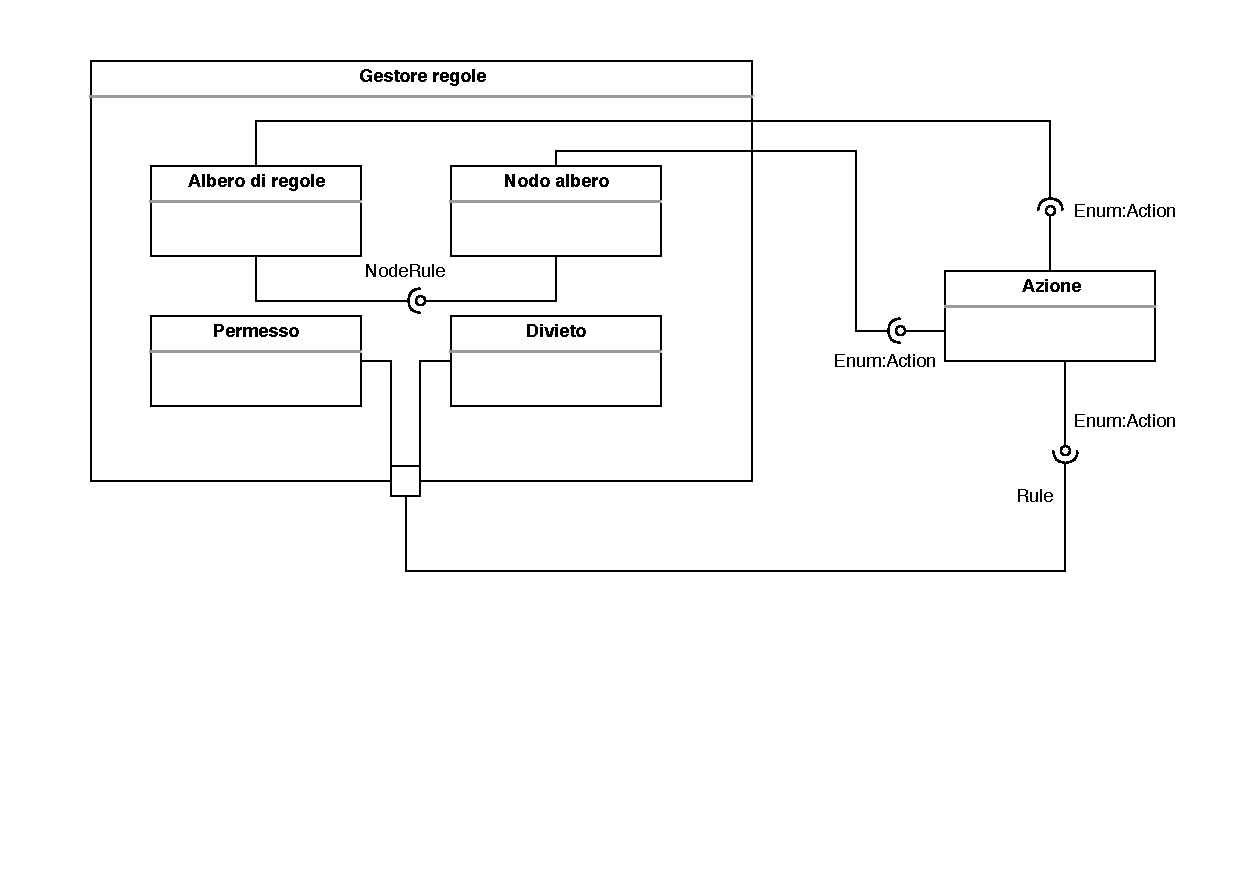
\includegraphics[scale=.60]{../immagini/imgCompRule}
\caption{Diagramma dei componenti per la rappresentazione delle regole}
\label{imgCompRule}
\end{figure}
Oltre ai componenti sopracitati, in figura è possibile vedere le implementazioni dell'interfaccia \textbf{Rule}, utilizzata per comunicare con il gestore della rappresentazione delle policy.
\paragraph{Creazione dell'albero}\mbox{}\\
L'albero viene creato dal suo gestore specificandone l'azione radice, tramite l'enumerativo \textbf{Action}. Come esposto nella sezione \ref{enumAction}, questo enumerativo permette di recuperare la lista delle azioni incluse dalla radice e, quindi, permette la creazione di eventuali sottoalberi. La creazione dei nodi figli è demandata al gestore del singolo nodo dell'albero.\\
Nel caso in cui, ad esempio, si andasse a specificare l'azione \textbf{use}, l'albero creato ha la seguente struttura:
\begin{itemize}
\item il nodo relativo all'azione \textbf{use} è la radice dell'albero;
\item tutte le azioni incluse da \textbf{use} compongono il livello successivo;
\item le azioni che a loro volta ne includono altre, come ad esempio \textbf{play}, sono le radici del sottoalbero corrispondente alla loro gerarchia;
\item risulta possibile notare come l'albero sia piatto, poiché un'azione generica tende ad avere molti figli, ma le azioni più specifiche tendono poi a non avere figli a loro volta.
\end{itemize}
\paragraph{Gestione dello stato di un'azione}\mbox{}\\
\label{ruleTree}
Ogni nodo dell'albero creato si riferisce ad una azione che può essere regolata e, oltre a tener conto della struttura gerarchica tra le azioni, rappresenta se l'azione si possa svolgere o meno. Gli stati in cui si può trovare un nodo sono 3:
\begin{enumerate}
\item \textbf{Permitted}: l'azione del nodo è permessa esplicitamente;
\item \textbf{Prohibited}: l'azione del nodo è proibita esplicitamente oppure tutte le sue azioni figlie sono nello stato \textbf{Prohibited};
\item \textbf{Undefined}: l'azione del nodo non ha regole che la interessano oppure era permessa ma almeno una azione figlia è \textbf{Prohibited} o \textbf{Undefined}.
\end{enumerate}
I singoli nodi si occupano anche di trasmettere lungo l'albero le conseguenze di un determinato cambio di stato:
\begin{enumerate}
\item settaggio a \textbf{Permitted}: il cambiamento viene propagato a tutti i nodi figli, a meno che:
\begin{itemize}
\item il nodo non fosse già nello stato \textbf{Prohibited}, in questo caso nessun settaggio viene svolto;
\item almeno uno dei nodi figli fosse nello stato \textbf{Prohibited}, in questo caso il nodo rimane  \textbf{Undefined}, mentre i nodi figli sui nodi figli si attua il settaggio a \textbf{Permitted};
\item il caso precedente si attua anche qualora uno dei nodi figli fosse \textbf{Undefined}.
\end{itemize}
\item settaggio a \textbf{Prohibited}: il cambiamento viene propagato a tutti i nodi figli, inoltre il nodo padre viene settato come \textbf{Undefined} se almeno un altro figlio non è ancora vietato, altrimenti anche il padre è settato come \textbf{Prohibited}; il passaggio del nodo padre ad \textbf{Undefined} è propagato fino alla radice della gerarchia;
\item settaggio a \textbf{Undefined}: questo settaggio avviene solamente come propagazione dai nodi figli nella casistica in cui non è necessario salire ulteriormente di livello.
\end{enumerate}
Di seguito alcuni esempi delle varie casistiche:
\begin{figure}[H]
\centering
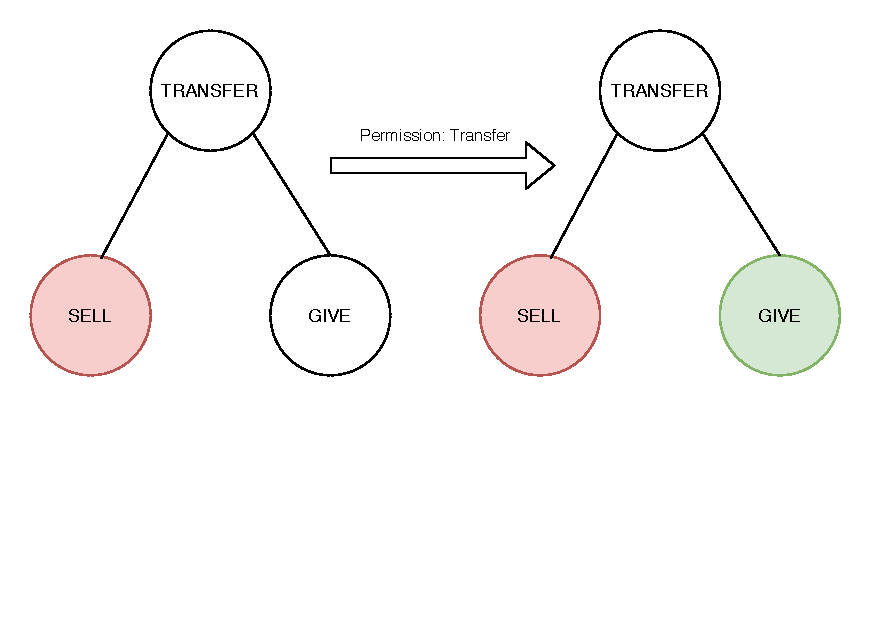
\includegraphics[scale=.50]{../immagini/propagationPerm}
\caption{Esempio di propagazione di un permesso, con azione figlia proibita}
\label{examplePerm}
\end{figure}
\begin{figure}[htp]
\centering
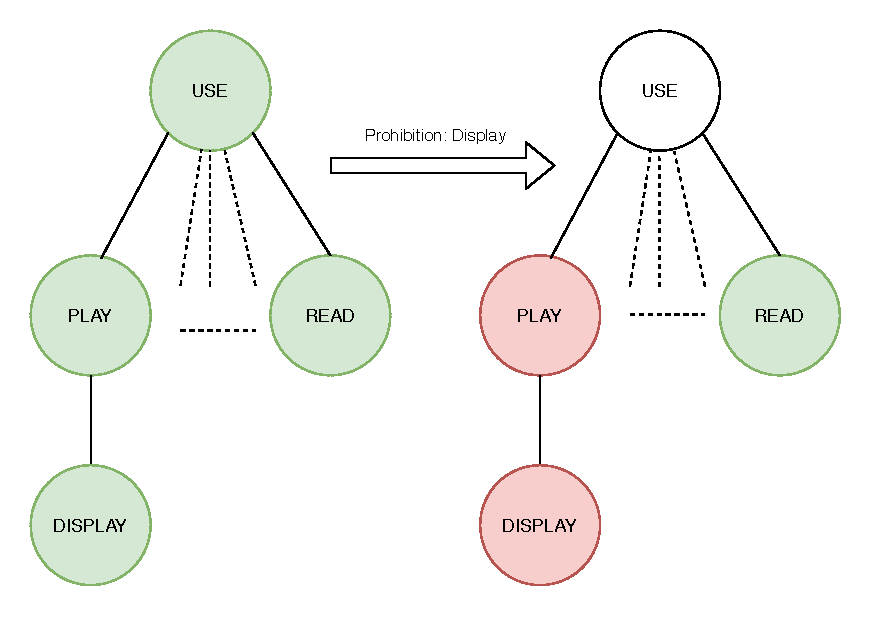
\includegraphics[scale=.50]{../immagini/propagationProParent}
\caption{Esempio di propagazione verso il padre di un divieto}
\label{exampleProParent}
\end{figure}

\paragraph{Recupero di un nodo e del suo stato}\mbox{}\\
L'albero creato non è un albero binario, di conseguenza la struttura dati in sé non supporta una ricerca efficiente dei nodi. La ricerca può essere resa però efficiente grazie alla gerarchia delle \textbf{Action} ed, in particolare, sfruttando l'enumerativo in figura \ref{imgActionEnum}, è possibile ricostruire il percorso che si deve fare da un nodo foglia alla radice per risalire alla gerarchia. Di seguito lo pseudo codice utilizzato per recuperare il nodo relativo ad un'azione:

\begin{lstlisting}[language=Json,firstnumber=1,caption={Il caso peggiore per questa ricerca è la profondità della gerarchia delle azioni. Il caso migliore si ha qundo l'azione non è nell'albero, con tempo di risposta costante.},label=listingAlgoNode,captionpos=b]
def getActionNode(Action a){
List steps = [];
Action visited = a;
Node exploredNode = Tree.getRoot();

while(visited != None){
  steps.add(visited);
  visited = visited.getFatherAction();
}

// Sempre vero a meno che non si chiami
// il metodo su un albero con radice errata
if(exploredNode.getAction() == steps.getLastStep()){
  steps.popLast();
  while(!(exploredNode.getAction() == a)){
  	exploredNode=
  	   visitedNode.getChildsMap()
  	     .get(steps.getLastStep);
  	steps.popLast();
  }
else{
  // Caso di albero con radice errata
  return null; 
}

return exploredNode;
                
}
\end{lstlisting}
Per il recupero dello stato relativo ad una azione, si usa il medesimo algoritmo mostrato nel listing \ref{listingAlgoNode} con un'ottimizzazione: qualora una delle azioni più in alto nella gerarchia fosse nello stato \textbf{Prohibited} o \textbf{Permitted}, si ritorna quello stato e si interrompe la ricerca del nodo, questo poiché:
\begin{itemize}
\item se l'azione più in alto nella gerarchia è \textbf{Permitted}, necessariamente tutte le azioni nel suo sottoalbero sono \textbf{Permitted}, se anche solo avesse uno stato diverso, la radice del sottoalbero sarebbe \textbf{Undefined} o \textbf{Prohibited};
\item  se l'azione più in alto nella gerarchia è \textbf{Prohibited}, anche il suo sottoalbero è \textbf{Prohibited}.
\end{itemize}
Le prestazioni nel caso peggiore rimangono comunque dipendenti dalla profondità della gerarchia delle azioni, mentre ai casi migliori si aggiunge lo scenario in cui l'azione radice dell'albero è \textbf{Prohibited} o \textbf{Permitted}: la casistica ha tempo d'esecuzione costante, come quella relativa all'azione non presente nell'albero.
\subsection{Rappresentazione Policy}\label{policyRappr}
Questa componente della rappresentazione attua le seguenti logiche:
\begin{itemize}
\item assegna ai target asset un insieme di regole;
\item le regole assegnate vengono rappresentate tramite 2 alberi delle regole: uno con radice \textbf{USE} ed uno con radice \textbf{TRANSFER};
\item si occupa di attuare il merging di 2 insiemi di regole;
\item le modalità di merging sono \textbf{intersect} e \textbf{union}.
\end{itemize}
\paragraph{Unione di policy}\mbox{}\\
L'unione di 2 policy è un'operazione creata per supportare uno scenario collaborativo, nel quale i permessi definiti da una policy vengono riconosciuti anche da quelli definiti da un'altra. Quest'operazione è attuata tramite i seguenti passi:
\begin{enumerate}
\item unione della lisa delle regole tra le regole della policy attuale e quella della policy con cui la si vuole unire;
\item creazione di una nuova policy avente il set di tutte le regole;
\item il metodo costruttore sfrutta la logica già esposta nel paragrafo \ref{ruleTree} relativo alla gestione degli alberi delle regole.
\end{enumerate}
\paragraph{Intersezione di policy}\mbox{}\\
L'intersezione di 2 policy è un'operazione creata per supportare uno scenario conservativo, nel quale non si ha controllo sui permessi definiti dalla policy con cui si effettua l'intersezione, di conseguenza un permesso è mantenuto solo nel caso in cui sia definito da entrambe le policy. La logica è attuata mediante i seguenti passi:
\begin{enumerate}
\item si recuperano gli stati relativi ad ogni azione in entrambe le policy; gli stati sono mantenuti in mappe con chiave l'azione regolata;
\item il passo 1 è attuato per entrambi gli alberi delle policy;
\item si itera una delle 2 mappe e si fanno i seguenti controlli:
\begin{itemize}
\item se l'azione è \textbf{Prohibited} in almeno una delle policy, si inserisce il divieto relativo tra le regole finali;
\item se l'azione è \textbf{Undefined} in almeno una delle policy, la si lascia non regolata;
\item se non si è nei due casi precedenti, l'azione allora è \textbf{Permitted} da entrambe e si inserisce il relativo permesso tra le regole finali;
\end{itemize}
\item si crea una nuova policy avente il set delle regole finali ottenute ai passi precedenti;
\item il metodo costruttore sfrutta la logica già esposta nel paragrafo \ref{ruleTree} relativo alla gestione degli alberi delle regole.
\end{enumerate}
\subsection{Rappresentazione Asset}\label{assetFun}
Questo componente si occupa di fornire funzioni relative alla gestione degli asset, le quali prevedono:
\begin{itemize}
\item supporto alla gerarchia degli asset, dando modo di esplicitare la proprietà \textbf{partOf}(attualmente la gerarchia è un albero, è possibile renderla un grafo a patto che non abbia cicli);
\item collega un asset alla policy che definisce delle regole ad esso relative;
\item propaga le regole di un asset alle collezioni figlie dell'asset, potendo scegliere come modalità di merging sia l'operazione \textbf{intersect} che quella di \textbf{union}, esposte in sezione \ref{policyRappr}.
\end{itemize}
Per supportare queste operazioni, si è usata un'architettura simile a quella delle regole mostrata nella sezione \ref{ruleRappr}, nella quale si sono separate le funzionalità a livello di gerarchia da quelle relative al singolo nodo. Di seguito è riportato il diagramma delle componenti:
\begin{figure}[H]
\centering
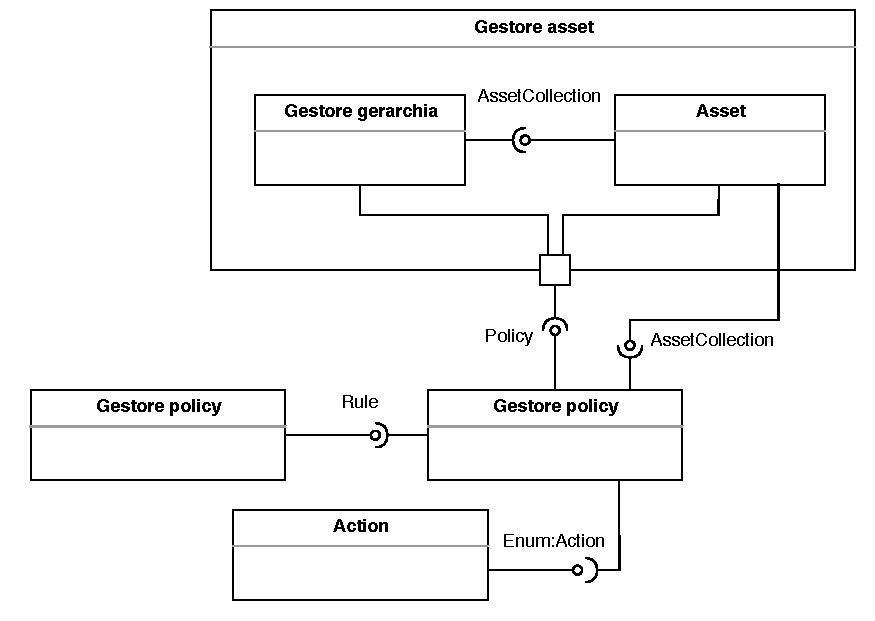
\includegraphics[scale=.7]{../immagini/compAsset.pdf}
\caption{Diagramma dei componenti per la rappresentazione degli asset}
\label{compAssetImg}
\end{figure}
Come è possibile notare dalla figura \ref{compAssetImg}, questo componente sfrutta la logica presente in ogni altro componente esposto precedentemente.\\
Lo scenario di utilizzo di un \textbf{Asset} si compone delle seguenti fasi:
\begin{enumerate}
\item definizione dei legami di gerarchia degli asset, seguento quanto esplicitato nella proprietà \textbf{partOf};
\item definizione delle regole relative all'asset;
\item creazione di una policy avente le regole definite al passo precedente;
\item assegnare la policy al gestore della gerarchia, il quale si occuperà di settare la policy per il nodo interessato e propagarla ai figli.
\end{enumerate}
\paragraph{Propagazione delle policy}\label{propagation}\mbox{}\\
La propagazione di una policy avviene dopo che questa è stata settata mediante la gerarchia: risulta quindi necessario recuperare il nodo; per questa prima fase dell'operazione si è utilizzata una ricerca in profondità, data la natura ricorsiva dell'operazione di propagazione; sarebbe stato possibile utilizzare anche una ricerca in ampiezza, ma il caso peggiore sarebbe rimasto il medesimo, data l'assenza di cicli.\\
Dopo il recupero del nodo interessato dalla policy, si attua l'effettiva propagazione ad ogni nodo figlio, fino ad arrivare ai nodi foglia. Qualora il nodo non avesse ancora una policy, viene settata quella del nodo padre.\\
Di seguito alcuni esempi:
\begin{figure}[H]
\centering
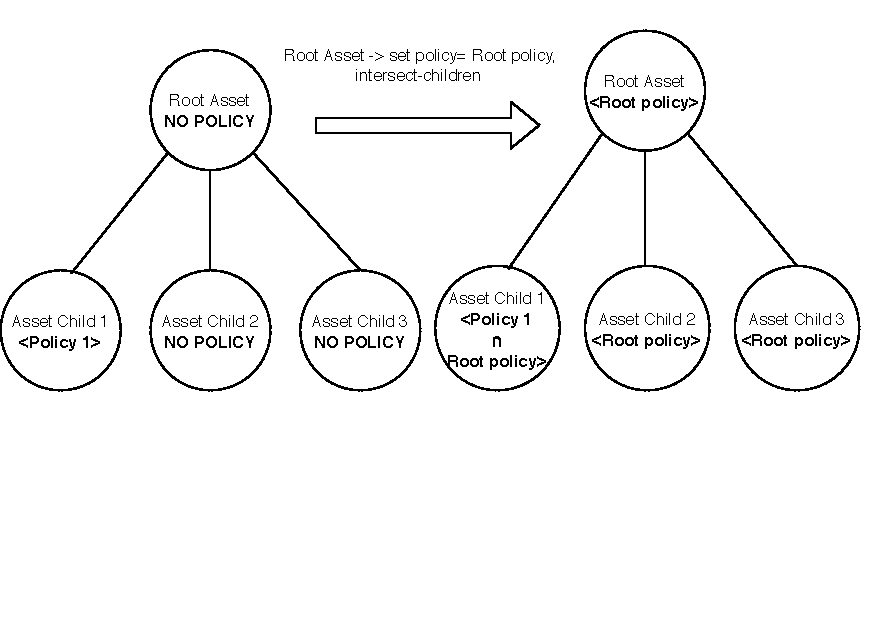
\includegraphics[scale=.70]{../immagini/assetSetPropagation.pdf}
\caption{Esempio di propagazione di una policy quando l'asset padre non ha policy, modalità con intersezione}
\label{imgAssetPropSet}
\end{figure}
\begin{figure}[H]
\centering
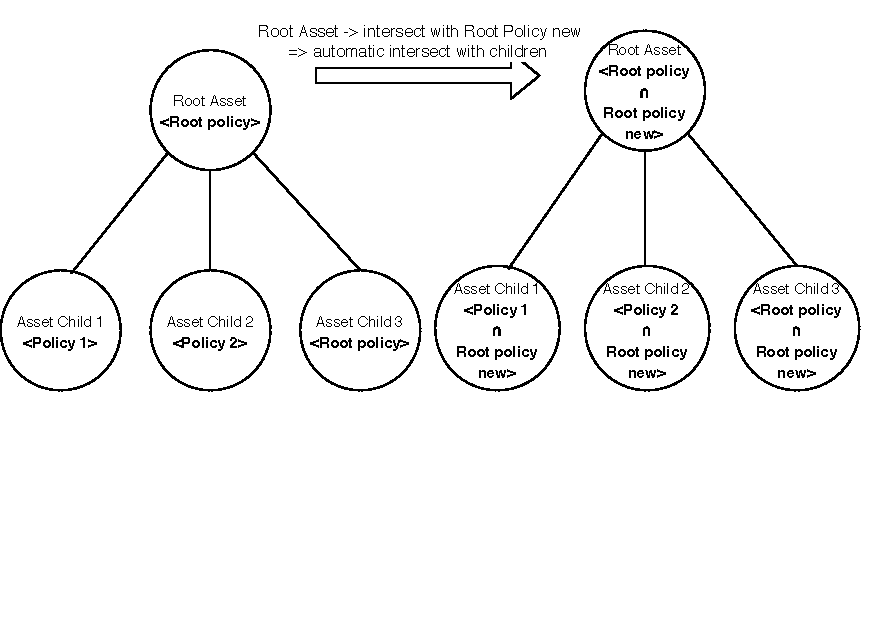
\includegraphics[scale=.70]{../immagini/assetIntersectPropagation.pdf}
\caption{Esempio di propagazione di una intersezione di policy}
\label{imgAssetPropIntersect}
\end{figure}
Il duale delle operazioni mostrate nelle figure \ref{imgAssetPropSet} e \ref{imgAssetPropIntersect} risulta disponibile per le operazioni di unione. Sempre dalla figura \ref{imgAssetPropIntersect} è possibile notare come se un asset figlio non abbia una propria policy, eredita in modo completo quella del nodo padre.
\paragraph{Recupero policy in seguito alla propagazione}\label{recuperoPolicy}\mbox{}\\
La policy relativo ad un nodo ai livelli più bassi può cambiare drasticamente in seguito ad una operazione di propagazione, come visibili nelle figure \ref{imgAssetPropSet} e \ref{imgAssetPropIntersect}. A supporto di altri componenti è stata implementata una procedura di recupero di policy del singolo nodo all'interno della gerarchia: si esplora in ampiezza l'intera gerarchia, recuperando ogni policy di ogni risorsa. Il risultato finale è una mappa che collega l'URI di ogni risorsa presente nella gerarchia alla sua policy; nel set di chiavi sono presenti anche i nodi non aventi una policy.
\subsection{Gestore procedura di merging}
TODO: Togliere semplificazioni dalla tesi: supporto a non propagare sull'intero DAG, albero non è più un DAG
Tutte le componenti fino ad ora mostrate si concentrano in modo atomico su una singola porzione della procedura del merging di 2 policy. Come è possibile notare supportano le operazioni di intersezione ed unione, ma tutte le strutture dati lavorano su un singolo documento ODRL. Il componente mostrato in questa sezione, invece, si occupa di attuare l'effettivo flusso applicativo desiderato. Di seguito il diagramma delle componenti che interessano il processo di merging:
\begin{figure}[H]
	\centering
	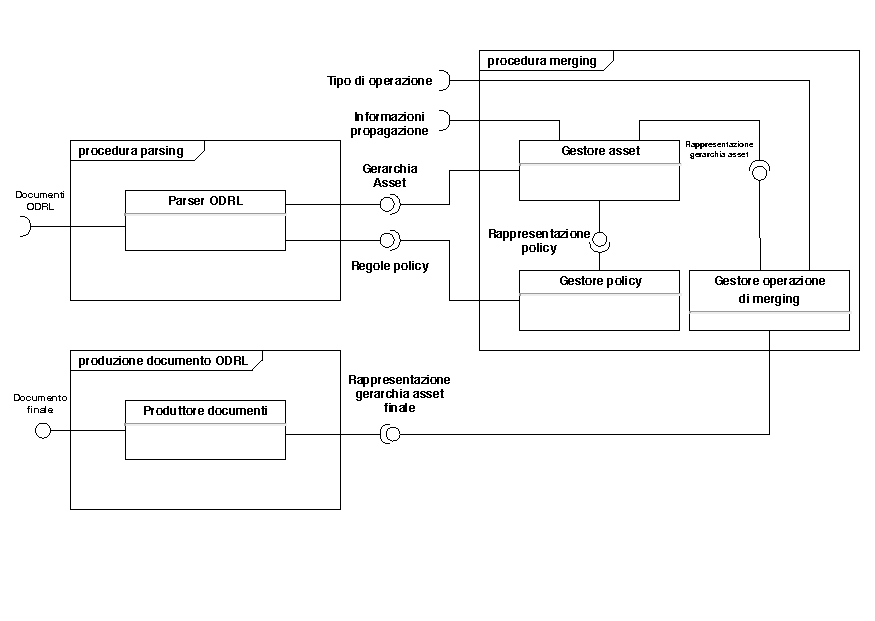
\includegraphics[scale=.70]{../immagini/processoMergin.pdf}
	\caption{Componenti che interagiscono nel processo di merging di 2 policy ODRL}
	\label{procMergin}
\end{figure}
Dalle interfacce esposte è possibile notare quali siano le informazioni che un utente deve specificare per attuare il merging di 2 policy:
\begin{itemize}
	\item i documenti contenenti le policy ODRL su cui si vuole operare;
	\item l'ambiente in cui le \textbf{singole} policy operano, identificato come:
	\begin{enumerate}
		\item \textbf{collaborativo}: la policy espressa in un asset ai livelli più alti della gerarchia si propaga in modalità \textbf{union} ai nodi ai livelli più bassi della gerarchia;
		\item \textbf{non collaborativo}: la policy espressa in un asset ai livelli più alti della gerarchia si propaga in modalità \textbf{intersection} ai nodi ai livelli più bassi della gerarchia;
	\end{enumerate} 
	\item l'operazione che si vuole attuare nel merging, che può essere \textbf{union} o \textbf{intersection};
	\item l'operazione decisa, applicherà il corrispondente ambiente operativo all'intera gerarchia che risultante dal merging delle 2 policy.
\end{itemize}
\paragraph{Casistiche supportate}\mbox{}\\
Tutti i casi di merging supportati, attualmente non prevedono un \textbf{Assignee} per le regole, si suppone quindi che tutte le regole si riferiscano allo stesso \textbf{Party} o \textbf{PartyCollection}. Un metodo per generalizzare queste casistiche per tener conto dell'\textbf{Assignee} delle regole sarebbe quello di creare una degli asset per ognuno degli attori interessati e ripetere i procedimenti di seguito per ognuno di loro.\\
Tenendo conto di questa prima semplificazione, il merging di 2 policy può essere attuato nei seguenti casi relativi alla gerarchia degli asset:
\begin{enumerate}
	\item le 2 policy regolano la medesima gerarchia di asset;
	\item le 2 policy regolano gerarchie totalmente disgiunte;
	\item una delle 2 policy regola l'intera gerarchia, mentre l'altra ne gestisce solo una porzione;
	\item una delle 2 policy inserisce nuovi nodi figli;
	\item una delle 2 policy inserisce un nuovo nodo padre.
\end{enumerate}
Tutte queste casistiche sono inoltre supportate per i seguenti scenari:
\begin{enumerate}
	\item intersezione di policy entrambe in ambiente collaborativo;
	\item intersezione di policy entrambe in ambiente non collaborativo;
	\item intersezione di policy in ambienti diversi;
	\item unione di policy entrambe in ambiente collaborativo;
	\item unione di policy entrambe in ambiente non collaborativo;
	\item unione di policy in ambienti diversi;
\end{enumerate}
\paragraph{Implementazione della procedura}\mbox{}\\
In questo paragrafo è riportata la procedura utilizzata per creare la rappresentazione della policy finale. All'interno dell'implementazione è stata usata la seguente semplificazione: le gerarchie degli asset sono alberi. Tale semplificazione è superabile implementando diversamente la rappresentazione degli asset al fine che sia possibile avere più di un unico parent node e verificando che il grafo ottenuto sia un \textbf{Directed acyclic graph} (\textbf{DAG}).
L'algoritmo può essere diviso nelle seguenti fasi:
\begin{enumerate}
	\item recupero della gerarchia complessiva regolata dalla policy finale, tale passo ha 2 sottopassi:
	\begin{enumerate}
		\item trattazione di asset presenti in entrambi i documenti di policy;
		\item trattazione di asset presenti in uno solo dei due documenti di policy;
	\end{enumerate}
	\item recupero delle 2 policy che descrivono ogni singolo asset all'interno della gerarchia;
	\item esecuzione dell'operazione desiderata su ogni asset;
	\item propagazione di tutte le policy ottenute all'interno della gerarchia degli asset finale, con ambiente coerente all'operazione effettuata.
\end{enumerate}
\subparagraph{Recupero gerarchia asset complessiva}\mbox{}\\
Di seguito gli pseudocodici relativi al recupero della gerarchia complessiva. Il primo passo riguarda il recupero degli asset in comune alle policy:
\begin{lstlisting}[language=Json,firstnumber=1,caption={L'algoritmo ha prestazioni lineari in proporzione al più più grande degli insiemi di asset},label=algoRecoverHierarchyComm,captionpos=b]
def Map<String, AssetCollection> mergeHierarchyCommon(
         Map<String,Asset> assetsFirst,
         Map<String,Asset> assetsSecond,
         AssetTree treeFirst,
         AssetTree treeSecond){
         
  Set uriSetFirst = assets.keySet();
  Set uriSetSecond = assetsSecond.keySet();
  Map<String, AssetCollection> finalAssets;
  commonURI = uriSetFirst.intersect(uriSetSecond);
  finalAssets.put("EveryAsset", everyAssetNode);
  for(String uri : commonURI){
  
    if(uri.equals("EveryAsset"))
      skip;  
    if(not(finalAssets.containsKey(uri)))
     finalAssets.put(uri,new Asset(uri));

    parentFirst = assetsFirst.get(uri).getParent();
    parentSecond = assetsSecond.get(uri).getParent();
    
    // Uno dei due non aveva un padre definito
    if(
    !parentFirst.getURI().equals(parentSecond.getURI()) && 
    (parentFirst.getURI().equals("EveryAsset") ||
     parentSecond.getURI().equals("EveryAsset"))){
       actParent =
        parentFirst.getURI().equals("EveryAsset") ?
        new Asset(parentSecond.getURI()) :
        new Asset(parentFirst.getURI());

       if(finalAssets.containsKey(actParent.getURI())){
        finalAssets.get(actParent.getURI()).addChild(finalAssets.get(uri));
       }else{
        actParent.addChild(finalAssets.get(uri));
        finalAssets.put(actParent.getURI(),actParent);
       }
    }
    
    //L'asset ha lo stesso padre in entrambe le policy
    if(parentFirst.getURI().equals(parentSecond.getURI())){
     if(finalAssets.containsKey(parentFirst.getURI())){
      finalAssets.get(parentFirst.getURI()).addChild(finalAssets.get(uri));
     }else {
      AssetCollection actParent = new Asset(parentFirst.getURI());
      actParent.addChild(finalAssets.get(uri));
      finalAssets.put(actParent.getURI(),actParent);
     }
    }
    return finalAssets;
  }
\end{lstlisting}
All'interno del listing \ref{algoRecoverHierarchyComm} è possibile notare:
\begin{itemize}
	\item all'interno delle casistiche relative agli asset in comune, non viene considerata la possibilità di asset con padri diversi poiché, lavorando con gerarchie espresse tramite alberi, questo porterebbe ad una situazione d'errore. Qualora si lavorasse con DAG, questa casistica porterebbe all'aggiunta di un nuovo parent node all'interno della lista dei parent del nodo esaminato;
	\item all'interno della gerarchia è inserito un asset avente URI \textbf{EveryAsset}; questo è un asset fittizio al quale non viene mai assegnata una policy, il suo ruolo è fungere da punto d'inizio per la ricerca degli asset che non hanno un parent esplicitato, al fine di avere un'unica sorgente nella ricerca.
\end{itemize}
Il passo sucessivo è il recupero degli asset non in comune:
\begin{lstlisting}[language=Json,firstnumber=1,caption={L'algoritmo ha prestazioni lineari in proporzione al numero di asset},label=algoRecoverHierarchyNotComm,captionpos=b]
def Map<String, AssetCollection> mergeHierarchyUniq(
       Map<String,Asset> assets,
       AssetTree tree,
       Map<String, AssetCollection> finalAssets){
       
 //In questo momento finalAsset contiene asset comuni      
 Set commonURI = finalAssets.keySet();  
 for(String uri: assets.keySet()){
   if(!commonURI.contains(uri)){
     if(!finalAssets.containsKey(uri))
      finalAssets.put(uri,new Asset(uri));
      
	 // Aggiunta parent similare ai comuni
     if(finalAssets.containsKey(assets.get(uri).getParentURI())){
       finalAssets.get(assets.get(uri).getParentURI()).addChild(finalAssets.get(uri));
     }else {
       AssetCollection actParent =
        new Asset(assets.get(uri).getParenttURI());
       actParent.addChild(finalAssets.get(uri));
       finalAssets.put(actParent.getURI(),actParent);
     }
   }
   return finalAssets;
 }
\end{lstlisting}
L'algoritmo esposto nel listing \ref{algoRecoverHierarchyNotComm} viene richiamato per gli insiemi di asset di entrambe le policy, coprendo così entrambi i set ricavabili dalle gerarchie.\\
Applicando i 2 algoritmi descritti finora, l'output presente in \textbf{finalAssets} sarà una mappa che collega ogni URI di un asset ad un oggetto che lo rappresenta che contiene già le informazioni riguardanti nodi parent e nodi figli. Sfruttando le componenti descritte nella sezione \ref{assetFun} è quindi possibile definire un \textbf{Gestore gerarchia} che ha come nodo sorgente \textbf{EveryAsset}; il gestore si occuperà di propagare le policy lungo la gerarchia.
\subparagraph{Recupero policy singole}\mbox{}\\
Come visibile all'interno del prototipo definito nel listing \ref{algoRecoverHierarchyComm}, il componente di parsing recupera le informazioni necessarie poiché un \textbf{Gestore gerarchia} possa creare una gerarchia di asset e propagare le varie regole relative alla policy; tutto questo seguendo le indicazioni relative all'ambiente definite dall'utente, come presentato in figura \ref{procMergin}.\\
Entrambe le policy originarie hanno un loro \textbf{Gestore gerarchia}, il quale si occupa di recuperare la policy di ogni nodo in seguito alla propagazione, la procedura è stata già presentata nella sezione \ref{recuperoPolicy}.\\
L'output di questo passo sono quindi 2 mappe, una per documento di policy, che legano l'URI di una risorsa alla policy ricavabile dal documento in cui è presente. 
\subparagraph{Esecuzione del merging e propagazione}\mbox{}\\
Gli ultimi due passi della procedura sono svolti iterando il set di chiavi della mappa \textbf{finalAssets} ottenuta in precedenza e recuperando entrambe le policy relative all'URI dell'asset dalle mappe ricavate al passo precedente. Risulta quindi possibile effettuare l'operazione di mergin desiderata, seguendo il corrispondente procedimento presentanto in sezione \ref{policyRappr} per poi propagare ogni policy lungo la gerarchia finale, come presentato nella sezione \ref{propagation}.\\
Il risultato finale è quindi un \text{Gestore gerarchia} dal quale possono essere recuperate tutte le policy finali relative agli asset. Queste policy vengono poi utilizzate dal produttore di policy per generare il documento ODRL relativo alle regole ottenute.
\section{Produzione policy ODRL}\label{produceSection}
//TODO
\bibliography{cit}{}
\bibliographystyle{plain}
\end{document}